\chapter{Channel Coding}

%--------- Intro ---------%
\section{Overview}
This part deals with linear block codes covering their fundamental concepts, generator and parity check matrices, error-correcting capabilities, encoding and decoding, and performance analysis. The linear block code discussed in this part is Hamming code.

\subsection{Shannon's Noisy Channel Coding Theorem}
Any channel affected by noise possesses a specific “channel capacity” C a rate of conveying information that can never be exceeded without error, but in principle, an error-correcting code always exists such that information can be transmitted at rates less than C with an arbitrarily low BER.

\subsection{Channel Coding Principle}
The channel coding principle is to add redundancy to minimize error rate as illustrated in Figure~\ref{fig:channel coding principle}.
\begin{figure}[ht]
    \centering
    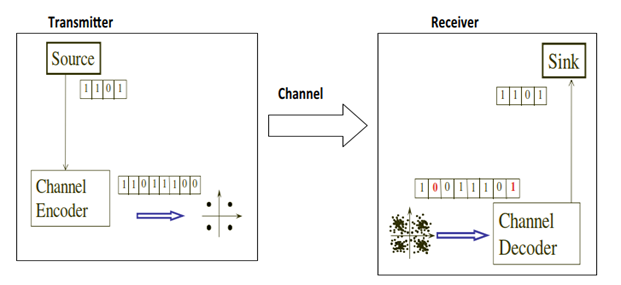
\includegraphics[width= 0.8\textwidth]{E1.PNG}
    \caption{Illustration of the channel coding principle.}
    \label{fig:channel coding principle}
\end{figure}

\subsection{Channel Coding Gain}
The bit error rate (BER) is the probability that a binary digit transmitted from the source received erroneously by the user. For required BER, the difference between the powers required for without and with coding is called the coding gain. A typical plot of BER versus Eb/No (bit energy to noise spectral density ratio) with and without channel coding is shown in Figure~\ref{fig:Coding gain}. It can be seen that coding can arrive at the same value of the BER at lower Eb/No than without coding. Thus, the channel coding yields coding gain which is usually measured in dB. Also, the coding gain usually increases with a decrease in BER.
\begin{figure}[ht]
    \centering
    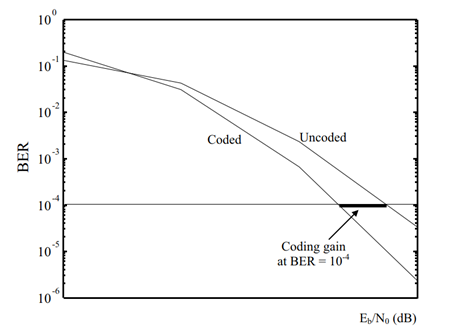
\includegraphics[width= 0.5\textwidth]{E2.PNG}
    \caption{Coding gain}
    \label{fig:Coding gain}
\end{figure}
%-------------------------%

%--------- Linear --------%
\section{Block Codes}
The data stream is broken into blocks of $k$ bits and each k-bit block is encoded into a block of n bits with $n > k$ bits as illustrated in Figure~\ref{fig:Coded data stream}. The n-bit block of the channel block encoder is called the code word. The code word is formed by adding $(n - k)$ parity check bits derived from the $k$ message bits.
\begin{figure}[ht]
    \label{}
    \centering
    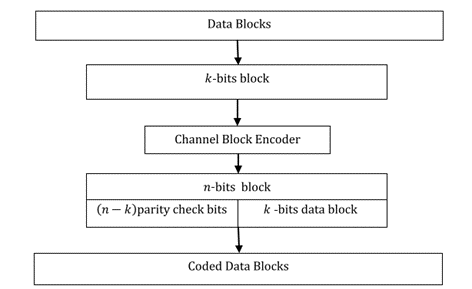
\includegraphics[width= 0.6\textwidth]{E3.PNG}
    \caption{Coded data stream}
    \label{fig:Coded data stream}
\end{figure}

\subsection*{Properties of Block Codes}

\subsubsection*{Block code rate}
The block code rate (R) is defined as the ratio of $k$ message bits and length of the code word $n$.
\[R = \frac{k}{n} \]

\subsubsection*{Code word weight}
The weight of a code word or error pattern is the number of nonzero bits in the code word or error pattern. \\
For example, the weight of a code word $c = (1, 0, 0, 1, 1, 0, 1, 0)$ is 4.

\subsubsection*{Hamming distance}
The Hamming distance between two blocks v and w is the number of coordinates in which the two blocks differ.
\[ d_{hamming}(v,w) = d(v,w) = | \{i | v_i \neq w_i, i = 0,1,\ldots,n-1 \} | \]
Example: Consider the code words $v$ = (00100) and $w$ = (10010), then the Hamming distance $d_{hamming}(v, w) = 3$. \\
Hamming distance allows for a useful characterization of the error detection and error correction capabilities of a block code as a function of the code's minimum distance.

\subsubsection*{The Minimum Distance of a Block Code}
The minimum distance of a block code $C$ is the minimum Hamming distance between all distinct pairs of code words in $C$.
\begin{GrayBox}
    \textbf{A code with minimum distance $d_{min}$ can:}
    \begin{itemize}
        \item \emph{detect} all error patterns of weight less than or equal to $(d_{min} - 1)$.
        \item \emph{correct} all error patterns of weight less than or equal to $(d_{min} - 1) / 2$.
    \end{itemize}
\end{GrayBox}
\textbf{Example:} Consider the binary code $C$ composed of the following four code words.
\[ C = \{(00100), (10010), (01001), (11111)\} \]
Hamming distance of (00100) and (10010) = 3 \\
Hamming distance of (10010) and (01001) = 4 \\
Hamming distance of (00100) and (01001) = 3 \\
Hamming distance of (10010) and (11111) = 3 \\
Hamming distance of (00100) and (11111) = 4 \\
Hamming distance of (01001) and (11111) = 3 \\
Therefore, the minimum distance $d_{min}$ = 3.

\subsection{Linear Block Codes}
A block code $C$ consisting of n-tuples $\{(c_0, c_1, . . . , c_{n-1})\}$ of symbols from $GF(2)$ is said to be binary linear block code if and only if $C$ forms a vector subspace over $GF(2)$. 
\begin{description}
    \item[Note:] finite fields are also called Galois fields (GF).
\end{description}
The code word is said to be systematic linear code word if each of the $2^k$ code words is represented as linear combination of $k$ linearly independent code words.

\subsubsection{Linear Block Codes Properties}
There are \emph{two important properties} of linear block codes which are:
\begin{description}
    \item[Property 1:] The linear combination of any set of code words is a code word.
    \item[Property 2:] The minimum distance of a linear block code is equal to the minimum weight of any nonzero word in the code.
\end{description}
Also, there are 2 well-known bounds on the minimum distance which are
\begin{description}
    \item[Singleton Bound:]
    The minimum distance of an $(n, k)$ linear code is bounded by
    \begin{equation}
        \label{eq:Singleton Bound}
        d_{min} \leq n-k+1
    \end{equation}
    \item[Hamming Bound:]
    An $(n, k)$ block code can \emph{detect} $t_{ed}$ errors per code word and can correct up to $t_{ec}$ errors per code word, provided that $n$ and $k$ satisfy the Hamming bound.
    \begin{equation}
        \label{eq:Hamming Bound}
        2^{n-k} \geq \sum_{i = 0}^{t_{ec}} \binom{n}{i} \quad \text{where} \quad \binom{n}{i} = \frac{n!}{(n-1)!i!}
    \end{equation}
    \[ t_{ec} = \frac{(d_{min} - 1)}{2} \quad , \quad t_{ed} = d_{min} - 1  \]
    The relation is the upper bound on $d_{min}$ and is known as \emph{the Hamming bound}.
\end{description}
 
\subsection{Generator \& Parity Check Matrices}
Let $\{g_0, g_1, \ldots  , g_{k-1}\}$ be a basis of code words for the $(n, k)$ linear block code $C$ and $m = [m_0, m_1, \ldots , m_{k-1}]$ the message to be encoded. The Theorem that says the code word $c = (c_0, c_1, \ldots , c_{n-1})$ for the message is uniquely represented by the following linear combination of $g_0, g_1, \ldots , g_{k-1}$
\[ c = m_0g_0 + \ldots + m_{k-1}g_{k-1} \]

for every code word $c \in C$.\\
Since every linear combination of the basis elements must also be a code word, there is a one-to-one mapping between the set of k-bit blocks $(a_0, a_1, \ldots , a_{k-1})$ over $GF(2)$ and the code words in $C$. A matrix $G$ is constructed by taking the vectors in the basis as its rows.
\[ G = \left[ \begin{array}{c}
    g_0 \\
    g_1 \\
    \vdots \\
    g_{k-1}
\end{array} \right] = \left[ \begin{array}{c c c c}
    g_{0,0} & g_{0,1} & \ldots & g_{0,n-1} \\
    g_{1,0} & g_{1,1} & \ldots & g_{1,n-1} \\
    \vdots & \vdots & \ddots & \vdots \\
    g_{k-1,0} & g_{k-1,1} & \ldots & g_{k-1,n-1}
\end{array} \right]
\]
This matrix $G$ is a generator matrix for the code $C$. It can be used to directly encode k-bit blocks in the following manner:
\[
mG = [m_0, m_1, \ldots, m_{k-1}] \cdot \left[ \begin{array}{c}
    g_0 \\
    g_1 \\
    \vdots \\
    g_{k-1}
\end{array} \right] = m_0g_0 + m_1g_1 + \ldots + m_{k-1}g_{k-1} = c
\]

The dual space of a linear block code $C$ is the dual code of $C$ and a basis $\{h_0, h_1, \ldots , h_{n-k-1}\}$ can be found for dual code of $C$, and the following parity check matrix can be constructed:
\[
H = \left[ \begin{array}{c}
    h_0 \\
    h_1 \\
    \vdots \\
    h_{n-k-1}
\end{array} \right] = \left[ \begin{array}{c c c c}
    h_{0,0} & h_{0,1} & \ldots & h_{0,n-1} \\
    h_{1,0} & h_{1,1} & \ldots & h_{1,n-1} \\
    \vdots & \vdots & \ddots & \vdots \\
    h_{n-k-1,0} & g_{n-k-1,1} & \ldots & g_{n-k-1,n-1}
\end{array} \right]
\]

In a systematic linear block code, the last $k$ bits of the codeword are \emph{the message bits}, that is
\[ c_i = m_{i-(n-k)} \quad , \quad i = n-k, \ldots , n-1 \]
While the first $n-k$ bits in the codeword are check bits generated from the k message bits according to
\[ c_0 = p_{0,0} m_0 + p_{1,0} m_1 + \ldots + p_{k-1, 0} m_{k-1} \]
\[ c_1 = p_{0,1} m_0 + p_{1,1} m_1 + \ldots + p_{k-1, 1} m_{k-1} \]
\[ \vdots \]
\[ c_{n-k-1} = p_{0,n-k-1} m_0 + p_{1,n-k-1} m_1 + \ldots + p_{k-1, n-k-1} m_{k-1} \]

The above equation can be written in a matrix form as:
\begin{equation}
    \label{equation:c=mG}
    [ c_0, c_1, \ldots, c_{n-1} ] = [ m_0, m_1, \ldots, m_{k-1} ] \left[ \begin{array}{c c c c c c c}
        p_{0,0} & p_{0,1} & \cdots & p_{0,n-k-1} & 1000 & \cdots & 0 \\
        p_{1,0} & p_{1,1} & \cdots & p_{1,n-k-1} & 0100 & \cdots & 0 \\
        \vdots & \vdots & \ddots & \vdots & \vdots & \vdots & \vdots \\
        p_{k-1,0} & p_{k-1,1} & \cdots & p_{k-1,n-k-1} & 0000 & \cdots & 1 \\     
    \end{array} \right]_{k \times n}
\end{equation}
\[ \text{or} \]
\[ c = mG \]
where $G$ is the matrix on the right hand side of the equation~\ref{equation:c=mG}. \\
The $k \times n$ matrix $G$ is called a generator matrix of the code and it has the following form:
\begin{equation}
    \label{eq:G}
    G = \left[ P | I_k \right]_{k \times n}
\end{equation}

The matrix $I_k$ is the identity matrix of order $k$, and $P$ is an arbitrary $k \times n-k $ matrix. When $P$ is specified, it defines the $(n, k)$ block code completely. The parity check matrix H corresponding to the above generator matrix G can be obtained as
\[ H = \left[ I_{n-k} | P^T \right] \]
\begin{equation}
    \label{equation:H}
    H = \left[ \begin{array}{c c c c c c c}
        1000 & \cdots & 0 & p_{0,0} & p_{0,1} & \cdots & p_{0,n-k-1} \\
        0100 & \cdots & 0 & p_{1,0} & p_{1,1} & \cdots & p_{1,n-k-1} \\
        \vdots & \vdots & \vdots & \vdots & \vdots & \ddots & \vdots \\
        0000 & \cdots & 1 & p_{0,n-k-1} & p_{1,n-k-1} & \cdots & p_{k-1,n-k-1} \\     
    \end{array} \right]
\end{equation}

\newtcbtheorem[auto counter,number within=section]{theo}
  {Theorem}{fonttitle=\bfseries\upshape, fontupper=\slshape,
     arc=0mm, colback=black!5!white,colframe=black!75!white}{theorem}

\begin{theo}{Parity Check Theorem}{}
    For any $(n, k)$ linear block code $C$ with $(n-k)\times n$ parity check matrix $H$, a code word $c \in C$ is a valid code word \textbf{if and only if} $cH^{T}=0$.
    \par\noindent\dotfill \\
    \textbf{Example:}\\
    For the following generator matrix of (7,4) block code. Find the code vector for the message vector m = (1110) and check the validity of code vector generated.
    \[
    G = \left[ \begin{array}{c c c | c c c c}
        1 & 1 & 0 & 1 & 0 & 0 & 0 \\
        0 & 1 & 1 & 0 & 1 & 0 & 0 \\
        1 & 1 & 1 & 0 & 0 & 1 & 0 \\
        1 & 0 & 1 & 0 & 0 & 0 & 1 
    \end{array} \right]
    \]
    \textbf{Solution:}\\
    The code vector for the message block $m = (1110)$ is given by
    \[
    c = mG = [1 1 1 0] \cdot \left[ \begin{array}{c c c | c c c c}
        1 & 1 & 0 & 1 & 0 & 0 & 0 \\
        0 & 1 & 1 & 0 & 1 & 0 & 0 \\
        1 & 1 & 1 & 0 & 0 & 1 & 0 \\
        1 & 0 & 1 & 0 & 0 & 0 & 1 
    \end{array} \right] = [0 1 0 1 1 1 0]
    \]
    \[
    H = \left[ \begin{array}{c c c | c c c c}
        1 & 0 & 0 & 1 & 0 & 1 & 1 \\
        0 & 1 & 0 & 1 & 1 & 1 & 0 \\
        0 & 0 & 1 & 0 & 1 & 1 & 1 
    \end{array} \right]
    \]
    \[
    cH^T = [0 1 0 1 1 1 0] \cdot \left[ \begin{array}{c c c}
        1 & 0 & 0 \\
        0 & 1 & 0 \\
        0 & 0 & 1 \\
        1 & 1 & 0 \\
        0 & 1 & 1 \\
        1 & 1 & 1 \\
        1 & 0 & 1 
    \end{array} \right] = [0 0 0]
    \]
    Hence, the generated code vector is valid.
\end{theo}

\section{Hamming Codes}
Hamming code is a linear block code capable of correcting single errors having a minimum distance $d_{min} = 3$. It is very easy to construct Hamming codes. The parity check matrix $H$ (obtained in equation~\ref{equation:H}) must be chosen so that no row in $H^T$ is zero and the first $(n-k)$ rows of $H^T$ form an identity matrix and all the rows are distinct. We can select $2^{n-k}-1$ distinct rows of $H^T$.\\
Since the matrix $H^T$ has $n$ rows, for all of them to be distinct, the following inequality should be satisfied.
\[ 2^{n-k} -1 \geq n \]
Implying that
\[ (n-k) \geq \log_2(n+1) \]
\begin{equation}
    \label{eq:n geq klog}
    n \geq k + \log_2(n+1)
\end{equation}
Hence, the minimum size $n$ for the code words can be determined from equation~\ref{eq:n geq klog}. \\

\textbf{Example:} Design a Hamming code with message block size of eleven bits. \\
\textbf{Solution:} It follows from equation~\ref{eq:n geq klog} that
\[ n \geq 11 + \log_2(n+1) \]
The smallest $n$ that satisfies the above inequality is 15, and hence, we need a $(15,11)$ block code. Thus, the transpose of the parity check matrix $H$ will be $4 \times 15$ matrix. The first four rows of $H^T$ will be $I_4$ matrix. The last eleven rows are arbitrarily chosen, with the restrictions that no row is zero, and all the rows are distinct.
\begin{equation}
    \label{eq:H solution}
    H^T = \left[ \begin{array}{c c c c}
        1 & 0 & 0 & 0 \\
        0 & 1 & 0 & 0 \\
        0 & 0 & 1 & 0 \\
        0 & 0 & 0 & 1 \\
        \hline
        0 & 1 & 0 & 1 \\
        0 & 1 & 1 & 0 \\
        0 & 1 & 1 & 1 \\
        0 & 0 & 1 & 1 \\
        1 & 0 & 0 & 1 \\
        1 & 0 & 1 & 0 \\
        1 & 0 & 1 & 1 \\
        1 & 1 & 0 & 0 \\
        1 & 1 & 0 & 1 \\
        1 & 1 & 1 & 0 \\
        1 & 1 & 1 & 1
    \end{array} \right] = \left[ \begin{array}{c}
        I_{n-k} \\
        \hline
        P^T    
    \end{array} \right]
\end{equation}

Then generator matrix $G$ equals
\[
G = \left[ \begin{array}{c c c c c c c c c c c c c c c}
    0&1&0&1&1&0&0&0&0&0&0&0&0&0&0 \\
    0&1&1&0&0&1&0&0&0&0&0&0&0&0&0 \\
    0&1&1&1&0&0&1&0&0&0&0&0&0&0&0 \\
    0&0&1&1&0&0&0&1&0&0&0&0&0&0&0 \\
    1&0&0&1&0&0&0&0&1&0&0&0&0&0&0 \\
    1&0&1&0&0&0&0&0&0&1&0&0&0&0&0 \\ 
    1&0&1&1&0&0&0&0&0&0&1&0&0&0&0 \\
    1&1&0&0&0&0&0&0&0&0&0&1&0&0&0 \\
    1&1&0&1&0&0&0&0&0&0&0&0&1&0&0 \\
    1&1&1&0&0&0&0&0&0&0&0&0&0&1&0 \\
    1&1&1&1&0&0&0&0&0&0&0&0&0&0&1
\end{array} \right]
\]

\textbf{Example:} Construct parity check and generator matrices for a $(7, 4)$ Hamming code. \\
\textbf{Solution:} The parity check matrix $H$ and generator matrix $G$ for a $(7, 4)$ Hamming code are
\[
H = \left[ \begin{array}{c c c c c c c}
    1 & 0 & 0 & 1 & 0 & 1 & 1 \\
    0 & 1 & 0 & 1 & 1 & 1 & 0 \\
    0 & 0 & 1 & 0 & 1 & 1 & 1
\end{array} \right]
\]
\[
G = \left[ \begin{array}{c c c c c c c}
    1 & 1 & 0 & 1 & 0 & 0 & 0 \\
    0 & 1 & 1 & 0 & 1 & 0 & 0 \\
    1 & 1 & 1 & 0 & 0 & 1 & 0 \\
    1 & 0 & 1 & 0 & 0 & 0 & 1
\end{array} \right]
\]

\subsection{Syndrome Table Decoding}
Consider a valid code word $c$ for transmission and let $e$ be an error pattern introduced by the channel during transmission. Then, the received vector $r$ can be written as
\[ r = c + e \]
Multiplying the $r$ by the transpose of the parity check matrix gives the syndrome $S$ which can be expressed as \\
\begin{equation}
    \label{eq:Syndrome Table Decoding}
    \begin{aligned}
        S &= r \cdot H^T \\
        &= (c+e) \cdot H^T \\
        &= cH^T + eH^T\\
        &= 0 + eH^T \\ 
        &= eH^T
    \end{aligned}
\end{equation}

Thus, the syndrome vector is independent of the transmitted code word $c$ and is only a function of the error pattern $e$. Decoding is performed by computing the syndrome of a received vector, looking up the corresponding error pattern, and subtracting the error pattern from the received word. \\

\textbf{Example:} Construct a syndrome decoding table for a $(7, 4)$ Hamming code \\
\textbf{Solution:} For a $(7, 4)$ Hamming code, there are $2^{(7-4)}$ error patterns $e$ as in Table~\ref{eq:Syndrome Table Decoding}
\begin{table}[!ht]
    \centering
    \caption{Syndrome decoding table for a $(7, 4)$ Hamming code}
    \label{tbl:syndrome decoding table}
    \begin{tabular}{cc}
        \toprule
        Error Pattern $e$ & Syndrome \\
        \midrule
        0000000 & 000 \\
        1000000 & 100 \\
        0100000 & 010 \\
        0010000 & 001 \\
        0001000 & 110 \\
        0000100 & 011 \\
        0000010 & 111 \\
        0000001 & 101 \\
        \bottomrule
    \end{tabular}
\end{table}

The syndrome for $(7, 4)$ Hamming code is computed using the parity check matrix $H$ (as given in the solution~\ref{eq:H solution}) as follows
\[ S = e \cdot H^T \]
Thus, the syndrome decoding table for a $(7, 4)$ Hamming code is as in Table~\ref{tbl:syndrome decoding table}

\subsection{Hamming Codes Decoding}
Syndrome table is used to decode the Hamming codes. The syndrome table gives the syndrome value based on the simple relationship with parity check matrix. The single-error-correcting codes (i.e., Hamming codes), are decoded by using syndrome value. Consider a code word $c$ corrupted by $e$, an error pattern with a single one in the $j^{th}$ coordinate position results a received vector $r$. Let ${h_0, h_1, \ldots , h_{n-1}}$ be the set of columns of the parity check matrix $H$. When the syndrome is computed, we obtain the transposition of the $j^{th}$ column of $H$. \\
\begin{equation}
    \label{eq:hamming codes decoding}
    s = eH^T = [0, \ldots, 0,1,0, \ldots, 0] \cdot \left[ \begin{array}{c}
        h_0^T \\
        h_1^T \\
        \vdots \\
        h_{n-1}^T
    \end{array} \right] = h_j^T
\end{equation}

The above-mentioned process in equation~\ref{eq:hamming codes decoding} can be implemented using the following algorithm:
\begin{enumerate}
    \item Compute the syndrome $s$ for the received word. If $s = 0$, the received code word is the correct code word.
    \item Find the position $j$ of the column of $H$ that is the transposition of the syndrome.
    \item Complement the $j^{th}$ bit in the received codeword to obtain the corrected code word. \\
\end{enumerate}

\textbf{Example:} Decode the received vector $r = [001100011100000]$ using the $(15,11)$ parity check matrix. \\
\textbf{Solution:} \\
\[
H = \left[ \begin{array}{c c c c c c c c c c c c c c c}
    1&0&0&0&0&0&0&0&1&1&1&1&1&1&1 \\
    0&1&0&0&1&1&1&0&0&0&0&1&1&1&1 \\
    0&0&1&0&0&1&1&1&0&1&1&0&0&1&1 \\
    0&0&0&1&1&0&1&1&1&0&1&0&1&0&1    
\end{array} \right]
\] \\
The received vector is $r = [001100011100000]$ \\
The corresponding syndrome $s = r \cdot H^T$ is \\
\[s = [0011]\] \\
The syndrome is the transposition of $7^{th}$ column of $H$. Inverting the $7^{th}$ coordinate of $r$, the following code word is obtained \\
\[c = [001100001100000]\]

\section{LDPC Coding}
Low density parity check (LDPC) codes are forward error-correction codes, invented by Robert Gallager in his MIT Ph.D. dissertation, 1960. The LDPC codes are ignored for long time due to their high computational complexity and domination of highly structured algebraic block and convolutional codes for forward error correction. A number of researchers produced new irregular LDPC codes which are known as new generalizations of Gallager's LDPC codes that outperform the best turbo codes with certain practical advantages. LDPC codes have already been adopted in satellite based digital video broadcasting and long-haul optical communication standards. This chapter discusses LDPC Code Properties, construction of parity check matrix for regular and irregular LDPC codes, efficient Encoding and Decoding of LDPC Codes, performance analysis of LDPC Codes.

\subsection{LDPC Code Properties}
Low Density Parity Check (LDPC) code is a linear error-correcting code that has a parity check matrix $H$, which is sparse i.e. with less nonzero elements in each row and column. LDPC codes can be categorized into regular and irregular LDPC codes. When the parity-check matrix $H_{(n - k)\times n}$ has the same number $w_c$ of ones in each column and the same number $w_r$ of once in each row, the code is a regular ($w_c$, $w_r$). The original Gallager codes are regular binary LDPC codes. The size of $H$ is usually very large, but the density of nonzero element is very low. LDPC code of length $n$, or denoted as an (n,$w_c$, $w_r$) LDPC code. Thus, each information bit is involved with $w_c$ parity checks, and each parity check bit is involved with $w_r$ information bits.\\
For a regular code, we have $(n-k)w_r = nw_c$ thus $w_c < w_r$.
\begin{equation}
    \label{eq:code rate}
    \begin{aligned}
        \text{code rate = } & \frac{(w_r - w_c)}{w_r} && \text{If all rows are linearly independent.} \\
        & \frac{k}{n} && \text{otherwise.}
    \end{aligned}
\end{equation}
Typically, $w_c \geq 3$. A parity check matrix with minimum column weight $w_c$ will have a minimum distance $d_{min} \geq w_c + 1$. When $w_c\geq 3$, there is at least one LDPC code whose minimum distance $d_{min}$ grows linearly with the block length $n$ thus a longer code length yields a better coding gain. Most regular LDPC codes are constructed with $w_c$ and $w_r$ on the order of 3 or 4.

\subsection{Construction of Parity Check Matrix H}
\subsubsection{Random Construction of H for Regular Codes}
In this method, the transpose of regular $(n, w_c, w_r)$ parity check matrix $H$ has the form
\[H^T =\begin{bmatrix}
H_{1}^T, H_{2}^T, ....., H_{wc}^T    
\end{bmatrix}\]
The matrix $H_1$ has $n$ columns and $\frac{n}{w_r}$ rows. The $H_1$ contains a single 1 in each column and contains 1s in its ith row from column $(i - 1)w_r + 1$ to column $i w_r$. Permuting randomly the columns of $H_1$ with equal probability, the matrices $H_2$ to $H_wc$ are obtained. The parity check matrix for $(n = 20, w_c = 3, w_r = 4)$ code constructed by Gallager is given as
\[H=\left[\begin{matrix}1\ 1\ 1\ 1\ 0\ 0\ 0\ 0\ 0\ 0\ 0\ 0\ 0\ 0\ 0\ 0\ 0\ 0\ 0\ 0\\0\ 0\ 0\ 0\ 1\ 1\ 1\ 1\ 0\ 0\ 0\ 0\ 0\ 0\ 0\ 0\ 0\ 0\ 0\ 0\\0\ 0\ 0\ 0\ 0\ 0\ 0\ 0\ 1\ 1\ 1\ 1\ 0\ 0\ 0\ 0\ 0\ 0\ 0\ 0\\0\ 0\ 0\ 0\ 0\ 0\ 0\ 0\ 0\ 0\ 0\ 0\ 1\ 1\ 1\ 1\ 0\ 0\ 0\ 0\\0\ 0\ 0\ 0\ 0\ 0\ 0\ 0\ 0\ 0\ 0\ 0\ 0\ 0\ 0\ 0\ 1\ 1\ 1\ 1\\1\ 0\ 0\ 0\ 1\ 0\ 0\ 0\ 1\ 0\ 0\ 0\ 1\ 0\ 0\ 0\ 0\ 0\ 0\ 0\\0\ 1\ 0\ 0\ 0\ 1\ 0\ 0\ 0\ 1\ 0\ 0\ 0\ 0\ 0\ 0\ 1\ 0\ 0\ 0\\0\ 0\ 1\ 0\ 0\ 0\ 0\ 0\ 0\ 1\ 0\ 0\ 0\ 1\ 0\ 0\ 0\ 1\ 0\ 0\\0\ 0\ 0\ 1\ 0\ 0\ 0\ 0\ 0\ 0\ 1\ 0\ 0\ 0\ 1\ 0\ 0\ 0\ 1\ 0\\0\ 0\ 0\ 0\ 0\ 0\ 0\ 1\ 0\ 0\ 0\ 1\ 0\ 0\ 0\ 1\ 0\ 0\ 0\ 1\\1\ 0\ 0\ 0\ 0\ 1\ 0\ 0\ 0\ 0\ 0\ 1\ 0\ 0\ 0\ 0\ 0\ 1\ 0\ 0\\0\ 1\ 0\ 0\ 0\ 0\ 1\ 0\ 0\ 0\ 1\ 0\ 0\ 0\ 0\ 1\ 0\ 0\ 0\ 0\\0\ 0\ 1\ 0\ 0\ 0\ 0\ 1\ 0\ 0\ 0\ 0\ 1\ 0\ 0\ 0\ 0\ 0\ 1\ 0\\0\ 0\ 0\ 1\ 0\ 0\ 0\ 0\ 1\ 0\ 0\ 0\ 0\ 1\ 0\ 0\ 1\ 0\ 0\ 0\\0\ 0\ 0\ 0\ 1\ 0\ 0\ 0\ 0\ 1\ 0\ 0\ 0\ 0\ 1\ 0\ 0\ 0\ 0\ 1\\\end{matrix}\right]\]

\subsubsection{Algebraic Construction of H for Regular Codes}
The construction of the parity check matrix $H$ using algebraic construction as follows [2, 3]. Consider an identity matrix $I_a$ where $a > (w_c - 1)(w_r - 1)$ and obtain the following matrix by cyclically shifting the rows of the identity matrix $I_a$ by one position to the right.
\[A^1=\left[\begin{matrix}0\ 1\ 0\ 0\ .\ .\ .\ .\ .\ .\ 0\\0\ 0\ 1\ 0\ .\ .\ .\ .\ .\ .\ 0\\0\ 0\ 0\ 1\ .\ .\ .\ .\ .\ .\ 0\\0\ 0\ 0\ 0\ .\ .\ .\ .\ .\ .\ 1\\1\ 0\ 0\ 0\ .\ .\ .\ .\ .\ .\ 0\\\end{matrix}\right]\]
Defining $A^0 = I_a$ the parity check matrix $H$ can be constructed as
\[H=\left[\begin{matrix}A^0&A^0&A^0&\ldots&A^0\\A^0&A^{1\ \ }&A^2&\ldots&A^{Wr-1}\\A^0&\ A^{2\ }&\ A^4&\ldots&A^{2(Wr-1)}\\\ &\ &\ &\ldots&\ \\A^0&\ A^{\left(Wc-1\right)\ \ }&A^{2(Wc-1)}&\ldots&A^{(Wc-1)(Wr-1)}\\\end{matrix}\right]\]

The constructed $H$ matrix has $w_ca$ rows and $w_ra$ columns, and it is of a regular ($w_ra$, $w_c$, $w_r$) having the same number of $w_r$ ones in each row and the same number of $w_c$ ones in each column. It is four cycle free construction. The algebraic LDPC codes are easier for decoding than random codes. For intermediate n, well designed algebraic codes yields a low BER.

\textbf{Example:} Construct H matrix with $w_c = 2$ and $w_r = 3$ using algebraic construction method.\\
\textbf{Solution} Since $(w_c - 1)(w_r - 1) = 2$
\[A=\left[\begin{matrix}A^0&A^1&A^0\\A^0&A^0&A^1\\A^1&A^0&A^0\\\end{matrix}\right]\]
\[H=\left[\begin{matrix}A^0&A^0&A^0\\A^1&A^1&A^1\\\end{matrix}\right]=\left[\begin{matrix}1\ 0\ 0\ 1\ 0\ 0\ 1\ 0\ 0\\0\ 1\ 0\ 0\ 1\ 0\ 0\ 1\ 0\\0\ 0\ 1\ 0\ 0\ 1\ 0\ 0\ 1\\1\ 0\ 0\ 0\ 1\ 0\ 0\ 0\ 1\\0\ 1\ 0\ 0\ 0\ 1\ 1\ 0\ 0\\0\ 0\ 1\ 1\ 0\ 0\ 0\ 1\ 0\\\end{matrix}\right]\]

\subsubsection{Random Construction of H for Irregular Codes}
In the random construction of the parity check matrix $H$ , the matrix is filled with ones and zeros randomly satisfying LDPC properties.\\
An example of parity check matrix for irregular LDPC code is
\[H=\left[\begin{matrix}1\ 1\ 0\ 1\ 1\ 0\ 0\ 1\ 0\ 0\\0\ 1\ 1\ 0\ 1\ 1\ 0\ 0\ 0\ 0\\0\ 0\ 0\ 1\ 0\ 0\ 0\ 1\ 1\ 1\\1\ 1\ 0\ 0\ 0\ 1\ 1\ 0\ 1\ 0\\0\ 0\ 1\ 0\ 0\ 1\ 0\ 1\ 0\ 1\\\end{matrix}\right]\]

\subsubsection{Representation of Parity Check Matrix Using Tanner Graphs}

The Tanner graph of the parity check matrix $H$ is a bipartite graph. It has bit nodes or variable nodes (VN) equal to the number of columns of $H$ , and check nodes (CN) equal to the number of rows of $H$. If $H_{ji}= 1$, i.e. if variable $i$ participates in the $j^{th}$ parity-check constraint, then check node $j$ is connected to variable node $i$.

\textbf{Example:} Construct Tanner graph for the following parity check matrix
\[H=\left[\begin{matrix}1\ 1\ 0\ 0\ 1\ 1\ 1\ 1\ 0\ 0\\1\ 0\ 1\ 1\ 0\ 1\ 0\ 1\ 0\ 1\\0\ 1\ 0\ 1\ 1\ 0\ 0\ 1\ 1\ 1\\1\ 0\ 1\ 0\ 1\ 0\ 1\ 0\ 1\ 1\\0\ 1\ 1\ 1\ 0\ 1\ 1\ 0\ 1\ 0\\\end{matrix}\right]\]
\textbf{Solution} The $H$ matrix has 10 columns and 5 rows. Hence, the associated tanner graph with 10 bit nodes and 5 check nodes is shown in Figure~\ref{fig:Tanner graph}.
\begin{figure}[h]
\centering
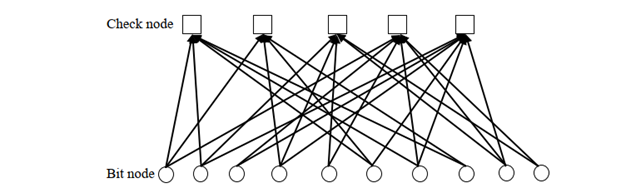
\includegraphics[width=6.47 in, height=2.01in]{27.PNG}
\caption{Tanner graph of $H$ matrix of the above example.}
\label{fig:Tanner graph}
\end{figure}

\subsection{LDPC Encoding}
\subsubsection{Preprocessing Method}
For coding purposes, we may derive a generator matrix $G$ from the parity check matrix $H$ for LDPC codes by means of Gaussian elimination in modulo-2 arithmetic. Since the matrix $G$ is generated once for a parity check matrix, it is usable in all encoding of messages. As such this method can be viewed as the preprocessing method. $1 \times n$ code vector $c$ is first partitioned as
\[C = [b : m]\]
where $m$ is $1 \times k$ message vector, and $b$ is the $1 \times n-k$ parity vector correspondingly, the parity check matrix $H$ is partitioned as
\[H^T=\left[\begin{matrix}H_1\\\ldots\\H_2\\\end{matrix}\right]\]
where $H_1$ is a square matrix of dimensions $(n - k)\times (n - k)$, and $H_2$ is a rectangular matrix of dimensions $k\times (n- k)$ transposition symbolized by the superscript T is used in the partitioning of matrix $H$ or convenience of representation. \\
Imposing the constraint $C H^T = 0$. \\
We may write
\[\left[b\ :\ m\right]\left[\begin{matrix}H_1\\ \ldots\\H_2\\\end{matrix}\right]=0\]
or equivalently
\[bH_1 + m H_2 = 0\]
The vectors $m$ and $b$ are related by
\[b = m P\]
where $P$ is the coefficient matrix. For any nonzero message vector $m$, the coefficient matrix of LDPC codes satisfies the condition
\[P H_1 + H_2 = 0\]
Which holds for all nonzero message vectors and, in particular, in the form $[0, \ldots, 0, 1, 0, \ldots, 0]$ that will isolate individual rows of the generator matrix. Solving the above Equation for matrix $P$, we get
\[P = H_2 H_{1}^{-1}\] 
where $H_{1}^{-1}$ is the inverse matrix of $H_1$, which is naturally defined in modulo-2 arithmetic. Finally, the generator matrix of LDPC codes is defined by
\[G = [P : I_k ] = [H_2 H_{1}^{-1} : I_k ]\]
where $I_k$ is the $k \times k$ identity matrix. The codeword can be generated as
\[C = mG\]

\textbf{Example:} Construct generator matrix $G$ for the following $(10, 3, 5)$ regular parity check matrix.
\[\left[\begin{matrix}1\ 1\ 0\ 1\ 0\ 1&\vdots&0\ 0\ 1\ 0\\0\ 1\ 1\ 0\ 1\ 0&\vdots&1\ 1\ 0\ 0\\1\ 0\ 0\ 0\ 1\ 1&\vdots&0\ 0\ 1\ 1\\0\ 1\ 1\ 1\ 0\ 1&\vdots&1\ 0\ 0\ 0\\1\ 0\ 1\ 0\ 1\ 0&\vdots&0\ 1\ 0\ 1\\0\ 0\ 0\ 1\ 0\ 0&\vdots&1\ 1\ 1\ 1\\\end{matrix}\right]\]
\textbf{Solution:}
\[H_1=\left[\begin{matrix}1\ 0\ 1\ 0\ 1\ 0\\1\ 1\ 0\ 1\ 0\ 0\\0\ 1\ 0\ 1\ 1\ 0\\1\ 0\ 0\ 1\ 0\ 1\\0\ 1\ 1\ 0\ 1\ 0\\1\ 0\ 1\ 1\ 0\ 0\\\end{matrix}\right]\ \ H_2=\left[\begin{matrix}0\ 1\ 0\ 1\ 0\ 1\\0\ 1\ 0\ 0\ 1\ 1\\1\ 0\ 1\ 0\ 0\ 1\\0\ 0\ 1\ 0\ 1\ 1\\\end{matrix}\right]\ \ \] 
\[H_1^{-1}=\left[\begin{matrix}0\ 0\ 1\ 0\ 1\ 1\\1\ 0\ 1\ 0\ 0\ 1\\1\ 1\ 1\ 0\ 0\ 0\\1\ 1\ 0\ 0\ 1\ 0\\0\ 1\ 0\ 0\ 1\ 1\\1\ 1\ 1\ 1\ 0\ 1\\\end{matrix}\right]\ \ \ \ \]
\[H_2H_1^{-1}=\left[\begin{matrix}0\ 1\ 0\ 1\ 0\ 1\\0\ 1\ 0\ 0\ 1\ 1\\1\ 0\ 1\ 0\ 0\ 1\\0\ 0\ 1\ 0\ 1\ 1\\\end{matrix}\right]\left[\begin{matrix}0\ 0\ 1\ 0\ 1\ 1\\1\ 0\ 1\ 0\ 0\ 1\\1\ 1\ 1\ 0\ 0\ 0\\1\ 1\ 0\ 0\ 1\ 0\\0\ 1\ 0\ 0\ 1\ 1\\1\ 1\ 1\ 1\ 0\ 1\\\end{matrix}\right]=\left[\begin{matrix}1\ 0\ 0\ 1\ 1\ 0\\0\ 0\ 0\ 1\ 1\ 1\\0\ 0\ 1\ 1\ 1\ 1\\0\ 1\ 0\ 1\ 1\ 0\\\end{matrix}\right]\ \ \ \ \ \]
The generator matrix
\[G = [H_2 H_{1}^{-1} : I_k ] =\left[\begin{matrix}1\ 0\ 0\ 1\ 1\ 0\ \vdots1\ 0\ 0\ 0\\0\ 0\ 0\ 1\ 1\ 1\ \vdots0\ 1\ 0\ 0\\0\ 0\ 1\ 1\ 1\ 1\ \vdots0\ 0\ 1\ 0\\0\ 1\ 0\ 1\ 1\ 0\ \vdots0\ 0\ 0\ 1\\\end{matrix}\right] \]

We will talk about the decoding of LDPC codes later in this chapter (Section~\ref{sec:LDPC decoding}).

\subsection{LDPC in 5G NR standards} 
Low-Density Parity-Check (LDPC) codes are linear error-correcting codes. According to the 3rd Generation Partnership Project (3GPP) TS 38.212, two channel coding codes, i.e., Polar codes and LDPC codes, are recommended for the Fifth-generation (5G) New Radio (NR). Polar codes are applied to 5G NR control channels. LDPC codes are suitable for 5G NR shared channels due to its high throughput, low latency, low decoding complexity and rate compatibility. \\
LDPC codes can be used to different block sizes with varying code rates because of the design of rate-compatible base graphs. Another advantage of 5G NR LDPC codes is that the performance of LDPC codes has an error floor around or below block error rate (BLER) 10-5 for all code sizes and code rates. \\
So LDPC codes play an important role in channel coding for 5G communication. Gallager invented LDPC codes in 1962 . \\
LDPC codes are linear block codes based on sparse parity-check matrix. It is forgotten for dozens of years because of the limited computation ability. In recent years, LDPC codes attract more attention because of their efficient decoding algorithms, excellent error-correcting capability, and their performance close to the Shannon limit for large code lengths. 5G needs to support high throughput up to 20 Gbps and a wide range of block sizes with different code rates for the data channels and hybrid automatic repeat request (HARQ). LDPC codes can fulfil the requirements. The base graphs defined in 3GPP TS 38.212 are structured parity-check matrix, which can efficiently support HARQ and rate compatibility that can support arbitrary amount of transmitted information bits with variable code rates. \\

LDPC plays a vital role in 5G NR. 5G technology has changed the way of people living in many aspects. We must build a digital trust society and comply with ethical requirements.
5G technology can help to reduce carbon emissions, as well as enable innovative applications in a range of sectors, from smart grid to precision agriculture, thereby helping to reduce CO2 emissions.

\subsubsection{Goals} 
The general objective of this part is to develop LDPC encoding and decoding chains, optimize LDPC encoding and decoding algorithms for implementing them on 5G. The specific objectives are to:
\begin{itemize}
    \item Understand the existing link level simulation code from 5G.
    \item Develop LDPC encoding and decoding chains according to 3GPP specification.
    \item Explore efficient LDPC encoding algorithm.
    \item Explore different LDPC decoding techniques.
    \item Optimize LDPC decoding algorithms for 5G NR shared channels.
    \item Implement optimized LDPC decoding algorithms on 5G.
    \item Evaluate the performance of algorithms in terms of BLER v.s. SNR graphs and execution CPU time.
    \item Discuss the benefits and drawbacks of the studied LDPC decoding algorithms with different code block sizes.
\end{itemize}

\subsubsection{NR Base graphs and parity-check matrix}
\textbf{Base graphs analysis}
In 3GPP TS 38.212 standard, there are two kinds of base graphs and their usage are determined by code rate and size of information bits. 
\begin{description}
    \item[Base graph 1:] 46 rows and 68 columns.
    \[K = 22Zc\]
    \item[Base graph 2:] 42 rows and 52 columns.
    \[K = 10Zc\]
\end{description}
Where $K$ is the maximum number of information bits, and $Z_c$ is the lifting size (expansion factor) shown in Table~\ref{tbl:ldpc lifting sizes}. There are 51 lifting sizes from 2 to 384 for each base graph.

\begin{tabularx}{0.8\textwidth} { | m{1em} | m{1cm}| m{1cm} | m{1em} | m{1cm}| m{1cm} | m{1em} | m{1cm}| m{1cm} | } 
    \hline
    $i_{LS}$ & 0 & 1 & 2 & 3 & 4 & 5 & 6 & 7 \\
    \hline
    a & 2 & 3 & 5 & 7 & 9 & 11 & 13 & 15 \\
    \hline
    $j_a$ & 7 & 7 & 6 & 5 & 5 & 5 & 4 & 4 \\
    \hline
\end{tabularx}
\[Z_c = a2^j \quad , \quad j = 0, \ldots ,j_a\]
\begin{table}[!ht]
    \centering
    \caption{LDPC lifting sizes}
    \begin{tabular}{ll}
        \toprule
        Set idex $(i_{LS})$ & Set of lifting sizes $(Z_c)$ \\
        \midrule
        0 & 2, 4, 8, 16, 32, 64, 128, 265 \\
        1 & 3, 6, 12, 24, 48, 96, 192, 384 \\
        2 & 5, 10, 20, 40, 80, 160, 320 \\
        3 & 7, 14, 28, 56, 112, 224 \\
        4 & 9, 18, 36, 72, 144, 288 \\
        5 & 11, 22, 44, 88, 176, 352 \\
        6 & 13, 26, 52, 104, 208 \\
        7 & 15, 30, 60, 120, 240 \\
        \bottomrule
    \end{tabular}
    \label{tbl:ldpc lifting sizes}
\end{table}

Both base graph 1 and base graph 2 have the same block structure shown in Figure~\ref{fig:block structure}. The columns include information columns, core parity columns, and extension parity columns. The rows are divided into core check rows and extension check rows.

\begin{figure}[h]
\centering
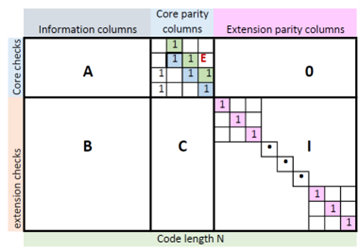
\includegraphics[width=3.75 in, height=2.6in]{29.PNG}
\caption{Base graphs block structure}
\label{fig:block structure}
\end{figure}

For base graph 1:
$A$ is a $4 \times 22$ matrix \\
$E$ is a $4 \times 4$ matrix \\
$0$ is $4 \times 42$ all zero matrix \\
$B$ is a $42 \times 22$ matrix \\
$C$ is a $42 \times 4$ matrix \\
$I$ is $42 \times 42$ identity matrix. \\

For base graph 2: \\
$A$ is a $4 \times 10$ matrix \\
$E$ is a $4 \times 4$ matrix \\
$0$ is $4 \times 38$ all zero matrix\\
$B$ is a $38 \times 10$ matrix \\
$C$ is a $38 \times 4$ matrix \\
$I$ is $38 \times 38$ identity matrix. \\

Sub-matrix E is a double diagonal matrix that is benefit for encoding. \\
An example of base graph 1 with set index iLS = 1 in 3GPP TS 38.212 standard is shown in Figure~\ref{fig:standard base graph 1}. In order to distinguish with the number 1 in base graphs in 3GPP TS 38.212 standard, -1 value in the base graph will be replaced by NULLS.

\begin{figure}[h]
\centering
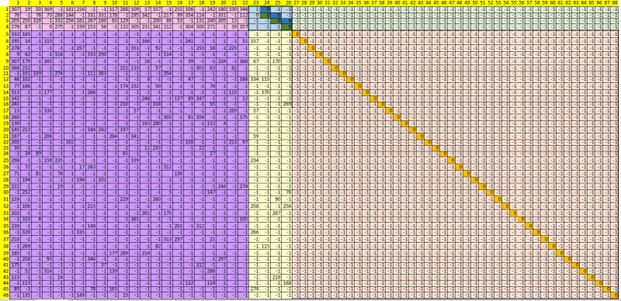
\includegraphics[width=6.47 in, height=3.14in]{30.PNG}
\caption{Base graph 1 with iLS = 1}
\label{fig:standard base graph 1}
\end{figure}

In 3GPP TS 38.212 standard, the base graphs correspond to maximum lifting size for each set index $i_LS$ shown in Table~\ref{tbl:ldpc lifting sizes}. For example, the base graph shown in Figure~\ref{fig:standard base graph 1} is the base graph with lifting size 384 corresponding to index $i_LS = 1$. The value of each element $P_i$, $j$ also known as circular shift value is from -1 to 383, which is a property of the base graph. The property is that circular shift value $P_{i,j}$ for base graph with arbitrary lifting size $Z_c$ ranges from $-1$ to $Z_c - 1$.

\textbf{Parity-check matrix calculation} \\
The parity-check matrix $H$ is obtained by replacing each element of base graph $H_BG$ with a $Z_c \times Z_c$ matrix, according to the following rules:
\begin{itemize}
    \item Each element of value $-1$ in $H_BG$ is replaced by an all zero matrix of size $Z_c \times Z_c$
    \item Each element of value $0$ in $H_BG$ is replaced by an identity matrix of size $Z_c \times Z_c$
    \item Each element of value from $1$ to $Z_c - 1$ in $H_BG$ which is denoted by $P_i$, $j$ is replaced by a circular permutation matrix $I$$(P_{i,j})$ of size $Z_c \times Z_c$, where $i$ and $j$ are the row and column indices of the element, and $I$$(P_{i,j})$ is obtained by circularly shifting the identity matrix $I$ of size $Z_c \times Z_c$ to the right $(V_{i,j})$ times. The main advantage of using a circularly shifting identity matrix is that it can reduce the memory requirement for implementation while also can facilitate the use of a simple switch network for encoding and decoding.
\end{itemize}

To simplify, a small example was used to explain the principle of how to get parity-check matrix $H$ (Figure~\ref{fig:H parity}). Assume that $B$ (Figure~\ref{fig:B}) is a base graph with lifting size 4.

\begin{figure}[h]
\centering
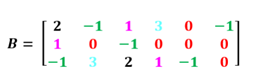
\includegraphics[width=2.65 in, height=0.82in]{31.PNG}
\caption{Base graph B}
\label{fig:B}
\end{figure}

\begin{figure}[h]
\centering
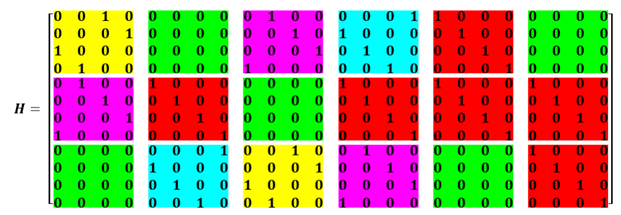
\includegraphics[width=6.47 in, height=2.24in]{32.PNG}
\caption{Parity-check matrix H}
\label{fig:H parity}
\end{figure}

\subsubsection{LDPC channel coding chain}
3GPP TS 38.212 standard defines the LDPC channel coding chain before the encoded information bits transmitted through the channel model. It is called LDPC encoding chain including 6 parts for both PUSCH and PDSCH. Figure~\ref{fig:coding chain} shows the LDPC encoding chain, which includes transport block CRC attachment, LDPC base graph selection, code block segmentation and code block CRC attachment, LDPC encoding, rate matching and code block concatenation. 

\begin{figure}[h]
\centering
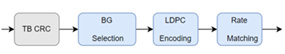
\includegraphics[width=0.75\textwidth]{33.PNG}
\caption{LDPC channel coding chain}
\label{fig:coding chain}
\end{figure}

\subsubsection{LDPC base graph selection}
LDPC base graph is selected based on the size of transport block (TB) message $A$ and transport block coding rate $R$. \\
If $A \leq 292$ , or if $A \leq 3824$ and $R \leq 0.67$ , or if $R \leq 0.25$ , LDPC base graph 2 is used. 
Otherwise, LDPC base graph 1 is used.

\subsection{Rate matching}
The purpose of rate matching is to adapt different code rates. \\
Rate matching is carried out on each code block independently. Assume that the input message to the $r_{th}$ code block is $d_1, d_2, \ldots , d_N$, where $N = 66Z_c$ for base graph 1 and $N = 50Z_c$ for base graph 2. $E_r$ is the length of rate matching output message of the $r_{th}$ code block. The output message after rate matching of the $r_{th}$ code block is $e_1, e_2, \ldots , e_{Er}$ which is calculated using equation
\[e_k = d_k, \qquad \text{if}\ d_k \neq \text{null},\ \text{where}\  1 \leq k \leq E_r\] 

In our project we make rate matching by puncturing as follows
\begin{equation}
    \label{eq:rate}
    \begin{aligned}
        R = & \frac{K}{n} \\
        = & \frac{K_bZ_c}{n_bZ_c} \\
        = & \frac{K_b}{n_b} \\
        K_b = & n_b - m_b
    \end{aligned}
\end{equation}

\begin{description}
    \item[$K_b$:] message bits(for base graph)
    \item[$n_b$:] code word length (for base graph) = columns of base graph
\end{description}
 
New columns after rate matching:
\begin{equation}
    \label{eq:New columns after rate matching}
    n_{bRM}=\left\lceil\frac{K_b}{R}\right\rceil
\end{equation}
New rows after rate matching:
\begin{equation}
    \label{eq:New rowa after rate matching}
    m_{bRM}=n_{bRM}-K_b
\end{equation}

\section{LDPC Decoding}
\label{sec:LDPC decoding}
LDPC decoding shown in Figure~\ref{fig:LDPC decoder} tries to correct errors using message iterative algorithms. There are two kinds of decoding algorithms for LDPC decoding. One decoding algorithm is called hard decision decoding, in which the message passed contains the actual value of bits, such as Bit Flipping Algorithm. The other decoding algorithm is called soft decision decoding, in which the message passed is the probability value associated with the occurrence of a particular bit. Soft decision decoding is based on the idea of belief propagation. For example, BP Algorithm is soft decision decoding. In this thesis project, soft decision decoding algorithms will be considered because soft decision decoding algorithms in the log domain provide better performance than hard decision decoding algorithms regardless of the SNR level.
\begin{figure}[ht]
    \centering
    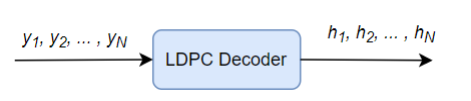
\includegraphics[width=0.5\textwidth]{image001.png}
    \caption{LDPC Decoder}
    \label{fig:LDPC decoder}
\end{figure}
The LDPC codes are generally decoded by the message-passing algorithms such as the belief propagation (BP) algorithm, which iteratively exchanges the messages through the edges between variable nodes and check nodes. \\
The BP algorithm achieves near-optimal decoding performance but suffers from high computational complexity. To find a better trade-off between performance and complexity, some efficient decoding algorithms are proposed using Min-Sum (MS) approximation. A simple algorithm for implementation is the Min-Sum Algorithm (MSA), but the outputs from variable nodes in MSA decoding are overestimated compared to SPA. There are many methods to optimize MSA including OMSA, linear approximation, self-corrected min-sum (SCMS) algorithms. A decoding scheme using the linear approximation and the modified message passing can achieve performance very close to that of the BP decoding. But it is difficult to hardware implementation because of heavy row weights. A hybrid algorithm for the LDPC codes in 5G, where the NMSA decoding and the linear approximation are applied has only a slight increase in complexity concerning the NMSA and improved performance much closer to the BP decoding, especially for the low-rate codes. We will focus on min-sum algorithm-MSA however, before we start, we need to know more about \emph{soft decision decoding} and \emph{log log-likelihood ratio (LLR)}.

\subsection{Important Concepts Before We Dig Deeper}
\subsubsection{Soft Decoding}
Soft decision decoding is a decoding technique used in error correction codes, such as forward error correction (FEC) codes. It involves making decisions about the transmitted data based on the received signal's strength or reliability, rather than relying solely on binary decisions (0 or 1).
In soft decision decoding, the received signal is typically represented as a continuous value, often referred to as a "soft metric" or "soft value." This soft metric represents the likelihood or probability of each possible transmitted symbol given the received signal.

Instead of making a hard decision and assigning a binary value to each symbol (e.g., 0 or 1), soft decision decoding takes into account the reliability of the received signal and assigns probabilities to different symbols. These probabilities are then used to make more accurate decisions about the transmitted data.

Soft decision decoding algorithms use various techniques, such as maximum likelihood estimation (MLE) or maximum a posteriori (MAP) estimation, to determine the most likely transmitted symbols based on the soft metrics. These algorithms consider not only the received signal but also statistical properties of the channel and noise characteristics.

Soft decision decoding can provide better error correction performance compared to hard decision decoding techniques, especially in channels with high noise levels or fading effects. By considering the reliability of each received symbol, soft decision decoding can effectively mitigate errors and improve overall system performance.

\subsubsection{Log Likelihood Ratio (LLR)}
The log-likelihood ratio (LLR) is a mathematical measure used in information theory and communication systems. It represents the logarithm of the ratio between the likelihoods of two competing hypotheses or decisions.
In soft decision decoding, LLR is important because it provides a way to quantify the reliability or confidence of a decision made by a receiver in a communication system. By using LLR, the receiver can make more informed and accurate decisions about the received signal.

The use of logarithm in LLR has several advantages:
\begin{description}
    \item[1. Compression:] Logarithms compress large dynamic ranges into smaller ones, making it easier to represent and process likelihood ratios.
    \item[2. Numerical stability:] Logarithms help avoid numerical underflow or overflow issues that may occur when dealing with very small or very large probabilities.
    \item[3. Additive property:] Logarithms convert multiplication operations into addition operations, simplifying calculations and reducing computational complexity. 
\end{description}
In soft decision decoding, LLR is used to estimate the likelihood that a particular transmitted symbol was received correctly. This information is then used to make more reliable decisions about the transmitted data, especially in scenarios where noise or interference may corrupt the received signal.

\subsubsection{Repetition Soft Input Soft Output Decoding}
We will take the $(3, 1)$ repetition code as example to explain repetition SISO decoder and we will assume BPSK representation of bits and AWGN channel.
\begin{figure}[h]
    \centering
    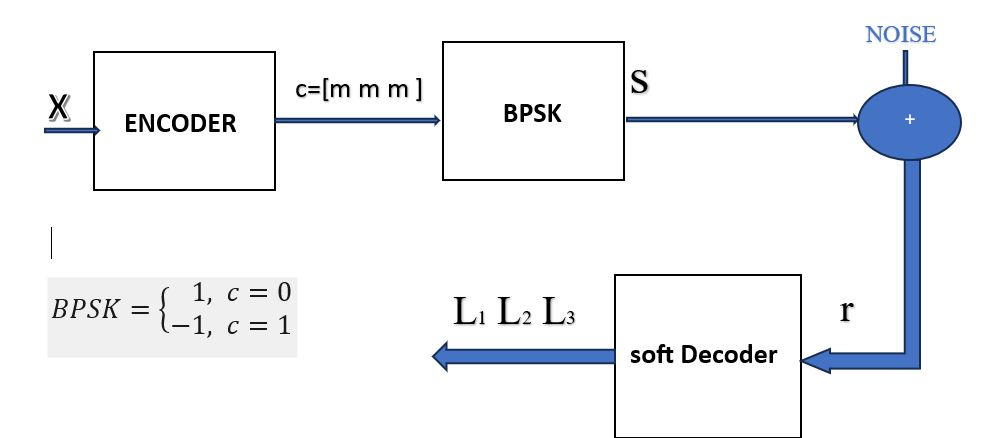
\includegraphics[width=0.55\textwidth]{ldpc_dec.jpg}
    \caption{Flow of Repetition Soft Input Soft Output Decoding}
    \label{fig:flow of LDPC RSISOD}
\end{figure}
We have a message bit $m$ okay it goes through the encoder, produce a code word which is $[m , m , m]$ , then we do BPSK we all know what it is by now $0 \rightarrow +1$, $1 \rightarrow -1$ and we get a symbol vector $S$ okay and then this goes through noise and get a receive vector $r$ which is $r_1, r_2, r_3$.\\
Using gaussian distributions
\[ p\left({\ r}_i\ \middle| c_i=0\right)=\frac{1}{\sqrt{2\sigma^2}}\ast e^{{-\frac{1}{{2\sigma}^2}({\ r}_i-1)}^2} \]
\[ p\left({\ r}_i\ \middle| c_i=1\right)=\frac{1}{\sqrt{2\sigma^2}}\ast e^{{-\frac{1}{{2\sigma}^2}({\ r}_i+1)}^2} \]
Using bay's theorem ,
\[p\left({\ r}_i\ \middle| c_i=0\right)=\frac{p\left({\ r}_i\ \middle| c_i=0\right).p(c_i=0)}{p(r_i)}\]
\[LLR=\log\frac{p\left(c_i=0\middle| r_i\right)}{p\left(c_i=1\middle| r_i\right)}\]
\[LLR=\frac{-1}{{2\sigma}^2}\left(\left(\ r_i-1\right)^2-\left(\ r_i+1\right)^2\right)\]
\[{LLR}_{intrinsic}= \frac{2}{\sigma^2} \ast r_i\]
\textbf{Note:} BPSK: $0 \rightarrow 1$ , $1 \rightarrow -1$.\\
$\frac{2}{\sigma^2}$ is a positive factor, practically in most cases we usually ignore this factor.\\

Output LLR (Beliefs $L$):
\[L_i=\log\frac{p\left(c_i=0\middle| r_{1,}r_2{,r}_3\right)}{p\left(c_i=1\middle| r_1{,r}_2,r_3\right)}\]
\[p\left(c_1=0\middle| r_1{,r}_2{,r}_3\right)=\frac{f\left(r_1{,r}_2{,r}_3\middle| c_1=0\right).p(c_1=0)}{f(r_1{,r}_2{,r}_3)}\]
\[p\left(c_1=1\middle| r_1{,r}_2{,r}_3\right)=\frac{f\left(r_1{,r}_2{,r}_3\middle| c_1=1\right).p(c_1=1)}{f(r_1{,r}_2{,r}_3)}\]
Assuming $p\left(c_1=0\right)=p\left(c_1=1\right)=.5$
\[\frac{p\left(c_1=0\middle| r_{1,}r_2{,r}_3\right)}{p\left(c_1=1\middle| r_1{,r}_2,r_3\right)}=\frac{f\left(r_1{,r}_2{,r}_3\middle| c_1=0\right)}{f\left(r_1{,r}_2{,r}_3\middle| c_1=1\right)}\]
When $c_1=0 \rightarrow S=[1 1 1] \rightarrow  r_1=1+N_1(0,\sigma^2)$ , $r_2=1+N_2(0,\sigma^2)$ , $r_3=1+N_3(0,\sigma^2)$: $N_1$, $N_2$, $N_3$ are \emph{independent}.
\[\frac{p\left(c_1=0\middle| r_{1,}r_2{,r}_3\right)}{p\left(c_1=1\middle| r_1{,r}_2,r_3\right)}=\frac{\exp \left( {\frac{{-(r_1-1)}^2}{{2\sigma}^2}}\right) \cdot \exp \left( {\frac{{-(r_2-1)}^2}{{2\sigma}^2}}\right) \cdot \exp \left( {\frac{{-(r_3-1)}^2}{{2\sigma}^2}}\right)}{\exp \left( {\frac{{-(r_1+1)}^2}{{2\sigma}^2}}\right)\cdot\exp \left( {\frac{{-(r_2+1)}^2}{{2\sigma}^2}}\right)\cdot\exp \left( {\frac{{-(r_3+1)}^2}{{2\sigma}^2}}\right)}=\exp \left( {\frac{2}{\sigma^2}(r_1+r_2+r_3)}\right)\]
\[L_1=log\frac{p\left(c_1=0\middle| r_{1,}r_2{,r}_3\right)}{p\left(c_1=1\middle| r_1{,r}_2,r_3\right)}=\frac{2}{\sigma^2}(r_1+r_2+r_3)\]
\[L_1=\frac{2}{\sigma^2}(r_1+r_2+r_3)\]
Intrinsic belief of $L_1=\frac{2}{\sigma^2}\ast r_1$ and extrinsic belief of $L_1=\frac{2}{\sigma^2}\ast(r_2+r_3)$ and it is valid for $L_{2},L_3 $.\\
The intrinsic belief that we have based on what we received for that symbol $r_1$ directly and then extrinsic what comes from $r_2$ and $r_3$ , so the intrinsic one is what we receive from the Channel corresponding to that particular symbol and extrinsic is what we gain or clean out of the other received values about this particle symbol.
We can generalize it Intrinsic belief of $L_i=\frac{2}{\sigma^2}\ast r_i$ and extrinsic belief of $L_i=\frac{2}{\sigma^2}\ast \sum \left( \text{other beleifs except }r_i \right)$
\[L_{i=}L_{intrinsic}+L_{extrinsic\ }\]
\begin{GrayBox}
    \textbf{Note:} Intrinsic belief is what we have based on what we received for that symbol $r_1$ directly and then extrinsic what comes from $r_2$ and $r_3$ so the intrinsic one is what we receive from the Channel corresponding to that particular symbol and extrinsic is what we gain or clean out of the other received values about this particle symbol.
\end{GrayBox}
Let us take simple example for illustration:
If we receive $r = [.01 -2.4 -1.5]$ the output from SISO decoder will be:
\[[L, L, L] = [-3.89, -3.89, -3.89] \ast \frac{2}{\sigma^2} \] 
( $\frac{2}{\sigma^2}$ :is a positive factor, practically in most cases we usually ignore this factor). 
Then we can apply hard decision $\rightarrow [1, 1, 1]$ (for BPSK).
\subsubsection{Single Parity Check Soft Input Soft Output Decoding}
A single parity-check code is a linear systematic code where a single parity-check is added at the end of the data word. Its generator and parity check matrices are :
\begin{equation*}
    G = \left[ \begin{array}{c c c c}
        1 & 0 & \cdots & 1 \\
        0 & 1 & \cdots & 1 \\
        \vdots & \vdots & \ddots & \vdots \\
        0 & 0 & \cdots & 1
    \end{array} \right] \qquad H = \left[ 1, 1, 1, \cdots, 1 \right]
\end{equation*}
For SPC$(n,n-1)$:\\
If $m=[m_1,m_2,m_3,m_4, \ldots, m_{n-1}]$, Encoder $\rightarrow  c=[ m_1,m_2,m_3,m_4, \ldots, m_{n-1}, p]$, where $p$:is the parity bit. $p = m_1 \oplus m_2 \oplus m_3 \oplus \ldots \oplus m_{n-1}$ (XOR of all massage bits).\\
\textbf{Example:} SPC$(3,2)$
\[C=\left[\begin{matrix}m_1&m_2&p\\0&0&0\\0&1&1\\1&0&1\\1&1&0\\\end{matrix}\right]\]
\textbf{Note:} we can consider each row as a possible code word and we noticed that number of 1's of any SPC code word is even. So, we can say that SPC code consist of all even weighted vectors of length $n$.\\
We will take the $(3, 2)$ SPC code as example to explain repetition SISO decoder and we will assume BPSK representation of bits and AWGN channel.
\begin{figure}[h]
    \centering
    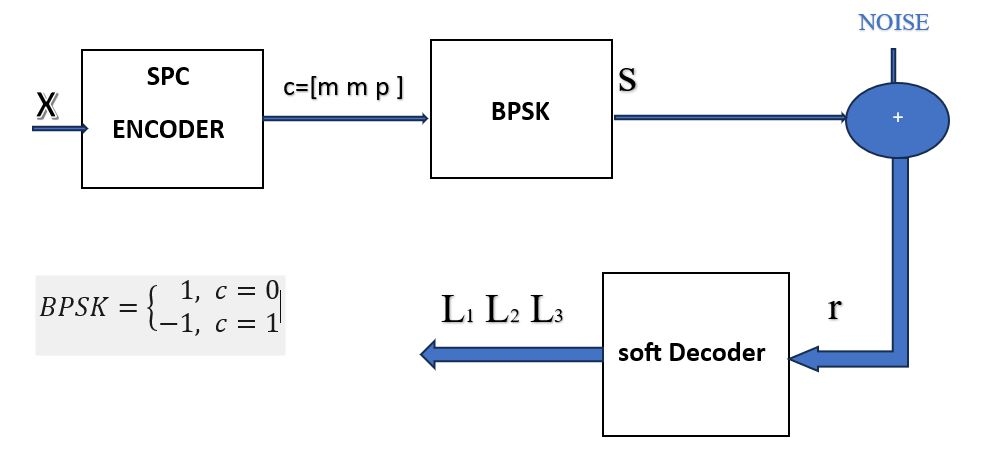
\includegraphics[width=0.55\textwidth]{ldpc_dec2.jpg}
    \caption{Flow of Single Parity Check Soft Input Soft Output Decoding}
    \label{fig:flow of LDPC SPC}
\end{figure}
We have a message bits $m_1$ and $m_2$ okay they go through the encoder, produce a code word which is $m_1 , m_2 , p$ , then we do BPSK we all know what it is by now 0 to +1, 1 to -1 and we get a symbol vector $S$ okay and then this goes through noise and get a receive vector $r$ which is $r_1, r_2, r_3$.\\
The output beliefs from decoder $L_1$, $L_2$ and $L_3$ 
\[L_{i}=l_\text{intrinsic}+l_\text{extrinsic}\]
To get the intrinsic belief we can do same calculation we have done before in repetition code and we will get same result:
\[l_{intrinsic(i)}=\frac{2}{\sigma^2}\ast r_i\]
The challenge here is to get extrinsic belief, we know now that $c_1 = c_2 \oplus c_3$\\
Let us say that: 
\[l_1=\log\frac{p\left(c_i=0\middle| r_{1,}\right)}{p\left(c_i=1\middle| r_1\right)}   	, p_1=p\left(c_1=0\middle| r_{1,}\right)\ \ \ \ \ ,p_2=p\left(c_2=0\middle| r_{2,}\right)\ \ ,p_3=p\left(c_3=0\middle| r_{3,}\right)\]
So we can say that:
\[l_1=\log\frac{p_1}{1-p_1}\]
And the same with $l_2$ and $l_3$.\\
Given $p_2, p_3$, what is $p(c1=0|r_2, r_3)$?
\[\begin{matrix}c1&c2&c3\\0&0&0\\0&1&1\\1&0&1\\1&1&0\\\end{matrix}\]
From previous table 
\[p_1=p_2\ p_3\ +\left(1-p_2\right)\left(1-p_3\right) \qquad (1)\]
\[1-p_1=p_2\ \left(1-p_3\right)+\left(1-p_2\right)p_3 \qquad (2)\]
$1-2:$
\[p_1-\left(1-p_1\right)=\left(p_2-\left(1-p_2\right)\right).(p_3-\left(1-p_3\right))\]
Using algebraic tricks:
\[\frac{p_1-\left(1-p_1\right)}{p_1+\left(1-p_1\right)}=\frac{\left(p_2-\left(1-p_2\right)\right)}{p_2+\left(1-p_2\right)}.\frac{(p_3-\left(1-p3\right))}{p_3+\left(1-p_3\right)}\]
\[\frac{1-\frac{1-p_1}{p_1}}{1+\frac{1-p_1}{p_1}}=\frac{1-\frac{1-p_2}{p_2}}{1-\frac{1-p_2}{p_2}}.\frac{1-\frac{1-p_3}{p_3}}{1-\frac{1-p_2}{p_2}}\]
\[l_{\text{extrinsic}(1)}=\log\frac{p_1}{1-p_1} \quad , \quad \frac{1-p_1}{p_1}=e^{-l_{extrinsic\ (1)}}\]
\[\frac{1-e^{-l_{extrinsic\ (1)}}}{1+e^{-l_{extrinsic\ (1)}}}=\frac{1-e^{-l_{(2)}}}{1+e^{-l_{\ (2)}}}.\frac{1-e^{-l_{(3)}}}{1+e^{-l_{\ (3)}}}\]
And we know that: 
\[\tanh{\left(x\right)}=\frac{e^x-e^{-x}}{e^x+e^{-x}}=\frac{1-e^{-2x}}{1+e^{-2x}} \quad,\quad l_{(2)}=\frac{2}{\sigma^2}\ast r_2\ \quad,\quad l_{(3)}=\frac{2}{\sigma^2}\ast r_3\]
$C_1=C_2 \oplus C_3 \rightarrow \tanh{\left(\frac{l_{extrinsic\ (1)}}{2}\right)=\tanh{\left(\frac{l_{(2)}}{2}\right) \cdot \tanh{\left(\frac{l_{(3)}}{2}\right)}}}$
Since tanh is an odd function it can be divided into absolute value and sign \\
Sign:			
\[\text{sign}\left(l_{extrinsic\ \left(1\right)}\right)=sign\left(l_{\left(2\right)}\right).sign(l_{\left(3\right)})\]
Absolute Value:
\[\tanh{\left(\frac{\left|l_{extrinsic\ (1)}\right|}{2}\right)=\tanh{\left(\frac{\left|l_{(2)}\right|}{2}\right).\tanh{\left(\frac{\left|l_{(3)}\right|}{2}\right)}}}\]
\[\log\tanh{\left(\frac{\left|l_{extrinsic\ (1)}\right|}{2}\right)=log\tanh{\left(\frac{\left|l_{(2)}\right|}{2}\right)+log\tanh{\left(\frac{\left|l_{(3)}\right|}{2}\right)}}}\]
Assume that:
\[x>0 \quad,\quad f\left(x\right)=\left|\log{\left(\tanh{\left(\frac{x}{2}\right)}\right)}\right|\]
\[f^{-1}\left(x\right)\approx f\left(x\right)\]
\[f\left(\left|l_{extrinsic\ \left(1\right)}\right|\right)=f\left(\left|l_{\left(2\right)}\right|\right)+f(\left|l_{\left(3\right)}\right|)\]
\[\left|l_{extrinsic\ \left(1\right)}\right|=f(f\left(\left|l_{\left(2\right)}\right|\right)+f\left(\left|l_{\left(3\right)}\right|\right))\]
\[ \left|l_{extrinsic\ \left(1\right)}\right|=f(f\left(\left|l_{\left(2\right)}\right|\right)+f\left(\left|l_{\left(3\right)}\right|\right)) \]
\begin{figure}[h]
    \centering
    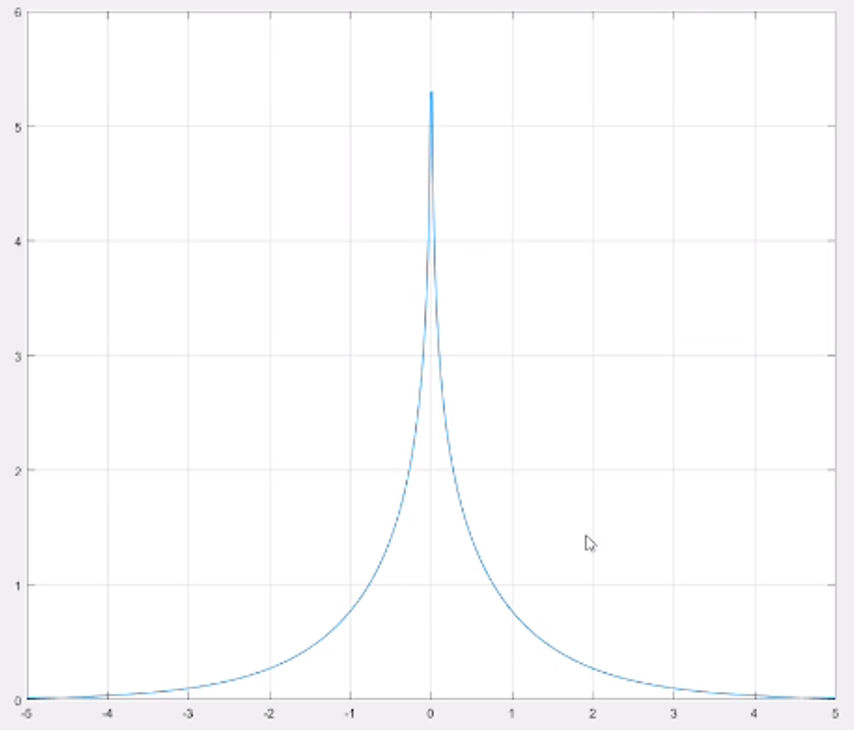
\includegraphics[width=0.4\textwidth]{tanh.png}
    \caption{f(x)}
    \label{fig:logtanh}
\end{figure}
Figure~\ref{fig:logtanh} shows $f\left(x\right)=|\log\left(\tanh{\left(\frac{x}{2}\right)}\right)|$. We can see that for small values of $x$ the value of $f(x)$ will be very large and for large values of $x$ the value of $f(x)$ will be very small so we can use very popular approximation for this this equation.
\[f(f\left(\left|l_{\left(2\right)}\right|\right)+f\left(\left|l_{\left(3\right)}\right|\right))\approx f(\min{\left(\left|l_{\left(2\right)}\right|,\left|l_{\left(3\right)}\right|\right)})\]
So we can say that 
\[\left|l_{extrinsic\ \left(1\right)}\right|=f(f(\min\left(\left|l_{\left(2\right)}\right|,\left|l_{\left(3\right)}\right|\right)))\]
\[f(f(\min\left(\left|l_{\left(3\right)}\right|,\left|l_{\left(2\right)}\right|\right)))\approx\min\left(\left|l_{\left(2\right)}\right|,\left|l_{\left(3\right)}\right|\right)\]
\[\left|l_{extrinsic\ \left(1\right)}\right|\approx\min\left(\left|l_{\left(2\right)}\right|,\left|l_{\left(3\right)}\right|\right)\]
And this is called \textbf{Min-Sum approximation}.
\begin{GrayBox}
    \[ \text{sign}\left(l_{extrinsic\ \left(1\right)}\right)=\text{sign}\left(l_{\left(2\right)}\right)\cdot \text{sign}(l_{\left(3\right)}) \]
    \[ \left|l_{\text{extrinsic} \left(1\right)}\right|\approx\min\left(\left|l_{\left(2\right)}\right|,\left|l_{\left(3\right)}\right|\right) \]
\end{GrayBox}
Now we can generalize these equations, if we have $n-1$ massage bits and the output code word length is $n$.
\[ l_{extrinsic\ \left(1\right)}=sign\left(l_{\left(2\right)}\right)\cdot sign\left(l_{\left(3\right)}\right) \cdot \ldots \cdot sign\left(l_{\left(n\right)}\right)\ast \min\left(\left|l_{\left(2\right)}\right|,\left|l_{\left(3\right)}\right|,\ldots,\left|l_{\left(n\right)}\right|\right) \]
\[ l_{extrinsic\ \left(2\right)}=sign\left(l_{\left(1\right)}\right)\cdot sign\left(l_{\left(3\right)}\right) \cdot \ldots \cdot sign\left(l_{\left(n\right)}\right)\ast \min\left(\left|l_{\left(2\right)}\right|,\left|l_{\left(3\right)}\right|,\ldots,\left|l_{\left(n\right)}\right|\right) \]
\[ l_{extrinsic\ \left(n\right)}=sign\left(l_{\left(1\right)}\right)\cdot sign\left(l_{\left(2\right)}\right) \cdot \ldots \cdot sign\left(l_{\left(n-1\right)}\right)\ast \min\left(\left|l_{\left(1\right)}\right|,\left|l_{\left(2\right)}\right|,\ldots,\left|l_{\left(n-1\right)}\right|\right) \]
instead of all these min we can do that:
\[ M_1=\min\left(\left|l_{\left(1\right)}\right|,\left|l_{\left(2\right)}\right|,\left|l_{\left(3\right)}\right|,\ldots,\left|l_{\left(n\right)}\right|\right) \]
where $M_1$ is the first absolute min.\\
\textbf{Where does first min occur?}\\
\textbf{Answer:}
\[ pos=\arg{\min\left(\left|l_{\left(1\right)}\right|,\left|l_{\left(2\right)}\right|,\left|l_{\left(3\right)}\right|,\ldots,\left|l_{\left(n\right)}\right|\right)} \]
\[ M_2=\min\left(\left|l_{\left(1\right)}\right|,\left|l_{\left(2\right)}\right|,\ldots,\left|l_{\left(pos-1\right)}\right|,\left|l_{\left(pos+1\right)}\right|,\ldots,\left|l_{\left(n\right)}\right|\right) \]
where $M_2$ is the second absolute min.
\[\left|l_{\text{extrinsic}\left(\text{pos}\right)}\right|=M_2\]
\[\left|l_{\text{extrinsic}\left(i\right)}\right|_{i\neq \text{pos}}=M_1\]
and assume that 
\[ S_{(\text{over all parity})}=sign\left(l_{\left(1\right)}\right) \cdot sign\left(l_{\left(2\right)}\right) \cdot sign\left(l_{\left(3\right)}\right)\cdot\ldots\cdot sign\left(l_{\left(n\right)}\right) \]
So we can say that
\[ sign\left(l_{extrinsic\ \left(1\right)}\right)=S \cdot sign\left(l_{\left(1\right)}\right) \]
\[ sign\left(l_{extrinsic\ \left(2\right)}\right)=S \cdot sign\left(l_{\left(2\right)}\right) \]
\[ sign\left(l_{extrinsic\ \left(n\right)}\right)=S \cdot sign\left(l_{\left(n\right)}\right) \]
And if
\begin{equation*}
    Sign\left(l_{extrinsic\ \left(1\right)}\right)
    \begin{cases}
        -Sign\left(l_{\ \left(i\right)}\right), & S < 0 \\
        Sign\left(l_{\ \left(i\right)}\right), & S > 0
    \end{cases}
\end{equation*}
Again, this approximation is very very important.\\
Repetition and single parity check (SPC) soft decoding are two important techniques used in LDPC belief propagation decoding. So, we need to know more about soft input soft output repetition and (SPC) decoding.
\begin{description}
    \item[Repetition:] In LDPC belief propagation decoding, repetition is used to improve the reliability of received bits. It involves transmitting the same information multiple times to increase the chances of correct reception. This redundancy helps in error detection and correction. By repeating the information, LDPC codes can achieve higher error correction capabilities.
    \item[Single Parity Check (SPC) Soft Decoding:] SPC is a simple error detection code that checks for parity errors in a block of data. In LDPC belief propagation decoding, SPC soft decoding is used as an initial step to estimate the likelihoods (or probabilities) of bit values based on received noisy signals. These likelihoods are then used as input to the belief propagation algorithm.
\end{description}
The belief propagation algorithm is a message-passing algorithm that iteratively updates the probabilities of bit values based on the received signals and the probabilities from neighboring bits. The SPC soft decoding provides an initial estimate of these probabilities, which helps in initializing the belief propagation process.\\
By combining repetition and SPC soft decoding with belief propagation, LDPC codes can achieve efficient error correction capabilities while maintaining low complexity. The repetition provides redundancy for error detection and correction, while SPC soft decoding helps in estimating initial probabilities for efficient belief propagation decoding.

\subsection{Message Passing Algorithm}
\subsubsection{Soft-Input Soft-Output Iterative Message Passing Decoder}
\begin{wrapfigure}{h}{0.4\textwidth}
    \centering
    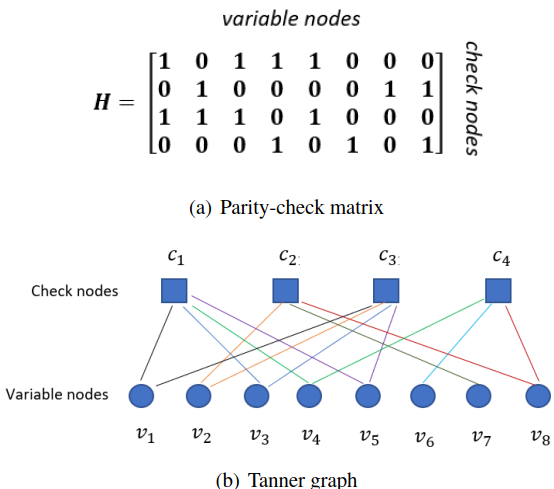
\includegraphics[width=0.4\textwidth]{image002.png}
    \caption{Parity Check Matrix and Tanner Graph}
    \label{fig:PCM and TG}
\end{wrapfigure}
LDPC codes can be represented using either parity matrix $H$ or Tanner graph introduced by Tanner. There are two sections in the tanner graph:
\textit{variable nodes} and \textit{check nodes} corresponding to rows and columns in the parity-check matrix. An example is shown in Figure~\ref{fig:PCM and TG}.

Tanner graph is an excellent way to illustrate iterative message passing decoding that messages are passed from variable nodes to check nodes, then from check nodes to variable nodes in each iteration. The message passing decoding can be divided into variable nodes operation, also called row operation, and check nodes operation, also called column operation. A message passing algorithm based on Pearl's belief algorithm describes the iterative decoding steps. There are different iterative message passing algorithms due to varying types of passed messages or different computations at the nodes, such as SPA and MSA. We will focus on MSA, LMSA and LOMSA. \\
One iteration of message passing can be divided into two parts.
One half-iteration is from variable nodes to check nodes shown in Figure~\ref{fig:variable and check nodes}(a),
in which all the information v1 has is sent to check node c3 except for the information
that check node c3 has already possessed. In this case, the information check node
c3 possesses is called extrinsic information. The other half iteration is from check
nodes to variable nodes, shown in Figure~\ref{fig:variable and check nodes}(b), in which check node c1 passes all
information it has available to it to each of the variable nodes vi excluding
the information the receiving node has already possessed. In this case, only information
consistent with c1 + c3 + c4 + c5 = 0 is sent. The message probability passed between
check nodes and variable nodes can be called belief, such as q13(b) in Figure~\ref{fig:variable and check nodes}(a).
\begin{figure}[ht]
    \centering
    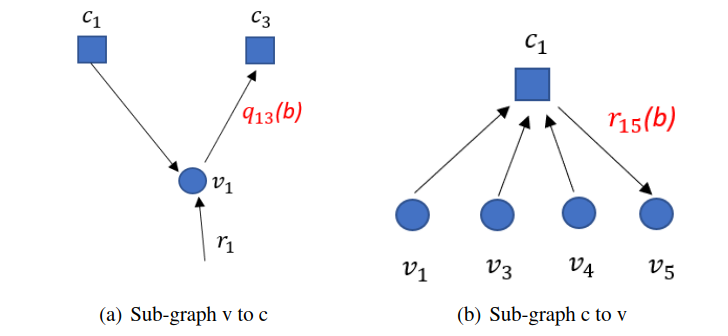
\includegraphics[width=0.55\textwidth]{image004.png}
    \caption{Iteration between variable nodes and check nodes}
    \label{fig:variable and check nodes}
\end{figure}

\subsubsection{Min-Sum Algorithm (MSA)} 
\begin{figure}[ht]
    \centering
    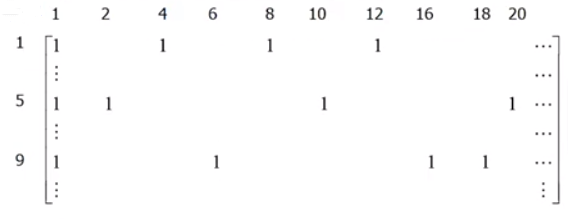
\includegraphics[width=0.4\textwidth]{image006.png}
    \caption{Part of an LDPC matrix}
    \label{fig:ldpc matrix}
\end{figure}

\begin{itemize}
    \item Use the received value corresponding to Bit 1
    \begin{itemize}
        \item $1^{st}$ estimate, $l_{10} = \text{LLR} | r_1 = \frac{2r_1}{\sigma^2}$
    \end{itemize}
    \item Use parity checks that involves the bit
    \begin{itemize}
        \item Row 1: $c_1 + c_4 + c_8 + c_{12} = 0$; $2^{nd}$ estimate, $l_{11} = \text{LLR} | r_4 , r_8 , r_{12}$
        \item Row 5: $c_1 + c_2 + c_{10} + c_{20} = 0$; $3^{rd}$ estimate, $l_{15} = \text{LLR} | r_2 , r_{10} , r_{20}$
        \item Row 9: $c_1 + c_6 + c_{16} + c_{18} = 0$; $4^{th}$ estimate, $l_{19} = \text{LLR} | r_6 , r_{16} , r_{18}$
    \end{itemize}
\end{itemize}

Figure~\ref{fig:tanner graph ldpc} shows the \textbf{first iteration} in tanner graph:
\begin{itemize}
    \item The first estimate $l_1$ comes from the channel
    \item $l_i$ : passed from bit node $i$ to all neighboring check nodes.
    \item Estimates for Bit 1: $l_{11}$, $l_{15}$, $l_{19}$ are calculated at check nodes $1$, $5$, $9$.
    \item Estimates passed from check nodes to neighboring bit nodes.
    \item This is done for all nodes in parallel.
\end{itemize}

\begin{figure}[ht]
    \centering
    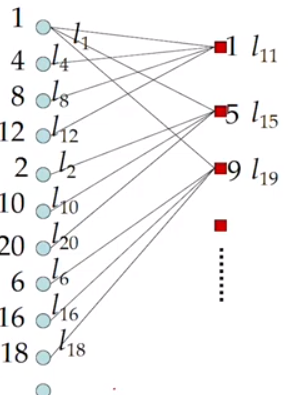
\includegraphics[width=0.25\textwidth]{image010.png}
    \caption{Tanner Graph}
    \label{fig:tanner graph ldpc}
\end{figure}

\begin{wrapfigure}{H}{0.35\textwidth}
    \centering
    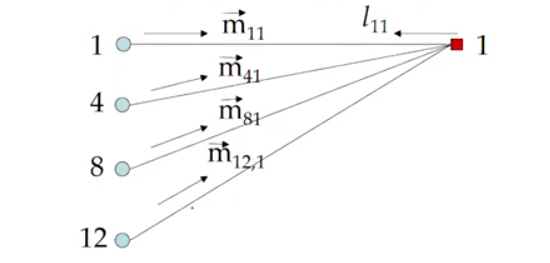
\includegraphics[width=0.35\textwidth]{image012.png}
    \caption{Second Iteration}
    \label{fig:ldpc iteration 2}
\end{wrapfigure}

\textbf{Second iteration:} check-to-bit (as shown in Figure~\ref{fig:ldpc iteration 2})
\begin{itemize}
    \item Repeat computation of $l_{11}$, $l_{15}$ and $l_{19}$ using $\overrightarrow{m_{41}}$, $\overrightarrow{m_{81}}$ and $\overrightarrow{m_{12,1}}$.
    \item Similar for all check nodes. 
\end{itemize}

\textbf{Summary of MSA} \\
\textbf{Row iteration:} \\
\begin{itemize}
    \item Check node computation (SPC SISO).
    \item Computes conditional LLRS for one bit.
\end{itemize}
\textbf{Column iteration:} \\
\begin{itemize}
    \item Bit node computation (Repetition SISO).
    \item Consolidate conditional LLRs.
\end{itemize}
Repeat for multiple iterations (as shown in Figure~\ref{fig:MSA})
\begin{figure}[ht]
    \centering
    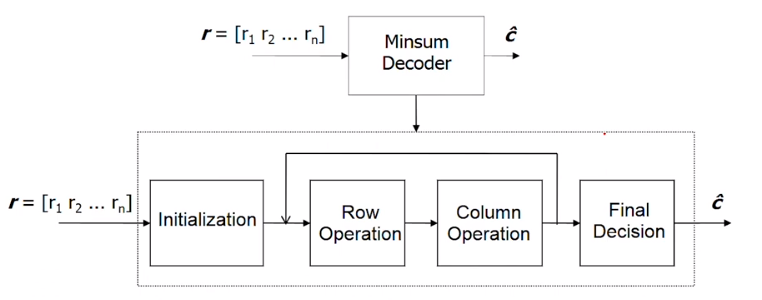
\includegraphics[width=0.6\textwidth]{image014.png}
    \caption{MSA}
    \label{fig:MSA}
\end{figure}
\textbf{Toy example for illustration:}\\
\[ H=\left[\begin{matrix}1&1&1&0&1&0&0\\0&1&1&1&0&1&0\\1&1&0&1&0&0&1\\1&0&1&0&1&1&1\\\end{matrix}\right] \]
We will use the above matrix for illustration. Typically , a much larger matrix is used in 5G !\\
\textbf{Storage matrix($L$)}:\\
$L$: Sparse matrix of same dimensions as parity-check matrix
\begin{itemize}
    \item NR, rate-1/2: $L$ is a $(22 \times 46) \times 48$ sparse matrix.
    \item For the toy example: $L$ is a $4 \times 7$ matrix.
    \item $L[i , j] = 0$ if $H[i , j] = 0$
    \item $L[i , j]$ can be nonzero only if $H[i , j] = 1$
\end{itemize}
\[ L=\left[\begin{matrix}x&x&x&0&x&0&0\\0&x&x&x&0&x&0\\x&x&0&x&0&0&x\\x&0&x&0&x&x&x\\\end{matrix}\right] \]
\textbf{1-Initialization Step}
\[ r= \left[\begin{matrix}r_1&r_2&r_3&r_4&r_5&r_6&r_7\\\end{matrix}\right] \]
\[ L=\left[\begin{matrix}r_1&r_2&r_3&0&r_5&0&0\\0&r_2&r_3&r_4&0&r_6&0\\r_1&r_2&0&r_4&0&0&r_7\\r_1&0&r_3&0&r_5&r_6&r_7\\\end{matrix}\right] \]
\[ r= \left[\begin{matrix}0.2&-0.3&1.2&-0.5&0.8&0.6&-1.1\\\end{matrix}\right] \]
\[ L=\left[\begin{matrix}0.2&-0.3&1.2&0&0.8&0&0\\0&-0.3&1.2&-0.5&0&0.6&0\\0.2&-0.3&0&-0.5&0&0&-1.1\\0.2&0&1.2&0&0.8&0.6&-1.1\\\end{matrix}\right] \]
\textbf{2-Row Operation: (SPC SISO)}
In-place computation using $L$, for each row:
\begin{itemize}
    \item Magnitude
    \begin{itemize}
        \item Min1 = minimum absolute value of all nonzero entries in row
        \item Min2 = next higher absolute value (second Min)
        \item Set magnitude of all values (except minimum (Min 1) = Min1)
        \item Set magnitude of minimum value (Min1) = Min2
    \end{itemize}
    \item Sign
    \begin{itemize}
        \item Parity = product of signs of entries in row
        \item New sign of an entry = (Old Sign) $\times$ (Parity)
    \end{itemize}
\end{itemize}
Row Operation on Row 1
\[ L=\left[\begin{matrix}-0.3&0.2&-0.2&0&-0.2&0&0\\0&-0.3&1.2&-0.5&0&0.6&0\\0.2&-0.3&0&-0.5&0&0&-1.1\\0.2&0&1.2&0&0.8&0.6&-1.1\\\end{matrix}\right] \]
After Row Operation On All Rows
\[ L=\left[\begin{matrix}-0.3&0.2&-0.2&0&-0.2&0&0\\0&-0.5&0.3&-0.3&0&0.3&0\\-0.3&0.2&0&0.2&0&0&0.2\\-0.6&0&-0.2&0&-0.2&-0.2&0.2\\\end{matrix}\right] \]
\textbf{3-Column Operation: (Repetition SISO)} \\
In-place computation using $L$, for each column:
\begin{itemize}
    \item New Values
    \begin{itemize}
        \item Sum j = r j+ sum of all entries in Column \[ Sum \rightarrow \text{updated values} \]
        \item New Entry = Sum - (Old entry)
    \end{itemize}
\end{itemize}
After Column Operation
\[ r_{old\ received\ values}=[\begin{matrix}0.2&-0.3&1.2&-0.5&0.8&0.6&-1.1\\\end{matrix}] \]
\[ L=\left[\begin{matrix}-0.3&0.2&-0.2&0&-0.2&0&0\\0&-0.5&0.3&-0.3&0&0.3&0\\-0.3&0.2&0&0.2&0&0&0.2\\-0.6&0&-0.2&0&-0.2&-0.2&0.2\\\end{matrix}\right] \]
\[ {Sum}_{updated\ values} = \begin{matrix} [-1&-0.4&1.1&-0.6&0.4&0.7&-0.7\\\end{matrix}] \]
\[ L_{new}=\left[\begin{matrix}-0.7&-0.6&1.3&0&0.6&0&0\\0&0.1&0.8&-0.3&0&0.4&0\\-0.7&-0.6&0&-0.8&0&0&-0.9\\-0.4&0&1.3&0&0.6&0.9&-0.9\\\end{matrix}\right] \]
Now, for the hard decision:
\begin{equation*}
    \text{BPSK}
    \begin{cases}
        1, & c=0 \\
        -1, & c=1
    \end{cases}
\end{equation*}
If $Sum > 0$, Decision on Bit $j = 0$, If $Sum < 0$, Decision on Bit $j = 1$.
\[ \begin{matrix}\text{sum}=[-1&-0.4&1.1&-0.6&0.4&0.7&-0.7\\\end{matrix}] \]
\[ \begin{matrix}\text{DEC}=[1&1&0&1&0&0&1\\\end{matrix}] \]

Same example can be represented using \emph{tanner graph}:\\
\textbf{1- Initialization Step}\\
Variable nodes sending messages to their connected check nodes. These messages contain information about the likelihood of each possible value of the variable given its neighboring check nodes.
\[ r=[\begin{matrix}0.2&-0.3&1.2&-0.5&0.8&0.6&-1.1\\\end{matrix}] \]
\begin{figure*}[ht]
    \centering
    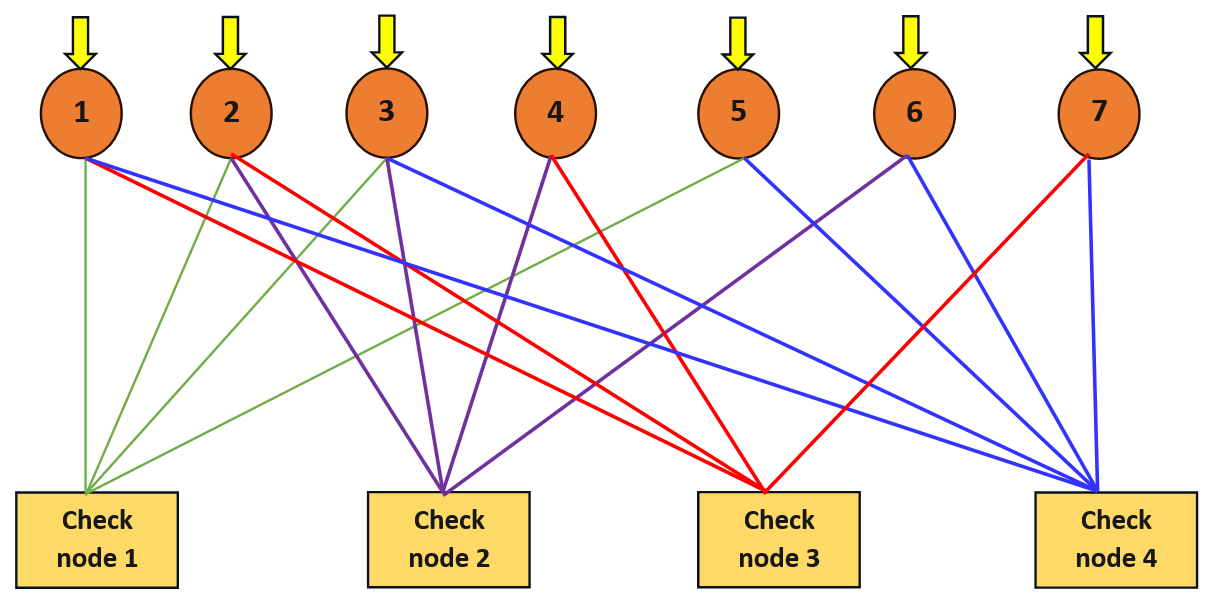
\includegraphics[width=0.55\textwidth]{46.png}
\end{figure*}

\textbf{2- Variable Node to Check Node:}\\
In first iteration each variable node has only the initial value so each variable node sends only the value of the variable node itself (initial value) however , after 1st iteration The message sent from variable node $i$ to check node $j$ is calculated as the sum of the incoming messages from all other neighboring check nodes except $j$, plus the value of the variable node itself. This can be represented as:
\[Message[i \rightarrow j] = Variable[i] + \sum(Message[k -> i]) \qquad \forall k \neq j \]
\begin{figure*}[ht]
    \centering
    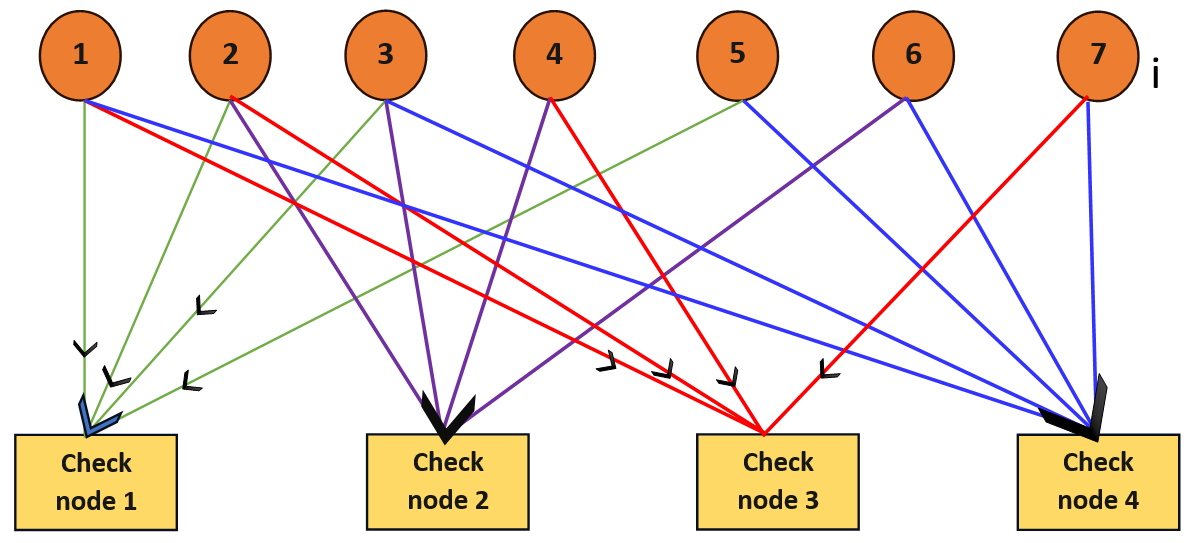
\includegraphics[width=0.55\textwidth]{47.png}
\end{figure*}

\textbf{3- Check to Variable Message Update:}\\
After receiving messages from all its neighboring variable nodes, each check node updates its outgoing messages to the variable nodes. The message sent from check node $j$ to variable node $i$ is calculated by Applying (Min-Sum) operation the operation on the incoming messages from all other neighboring variable nodes.
\begin{figure*}[ht]
    \centering
    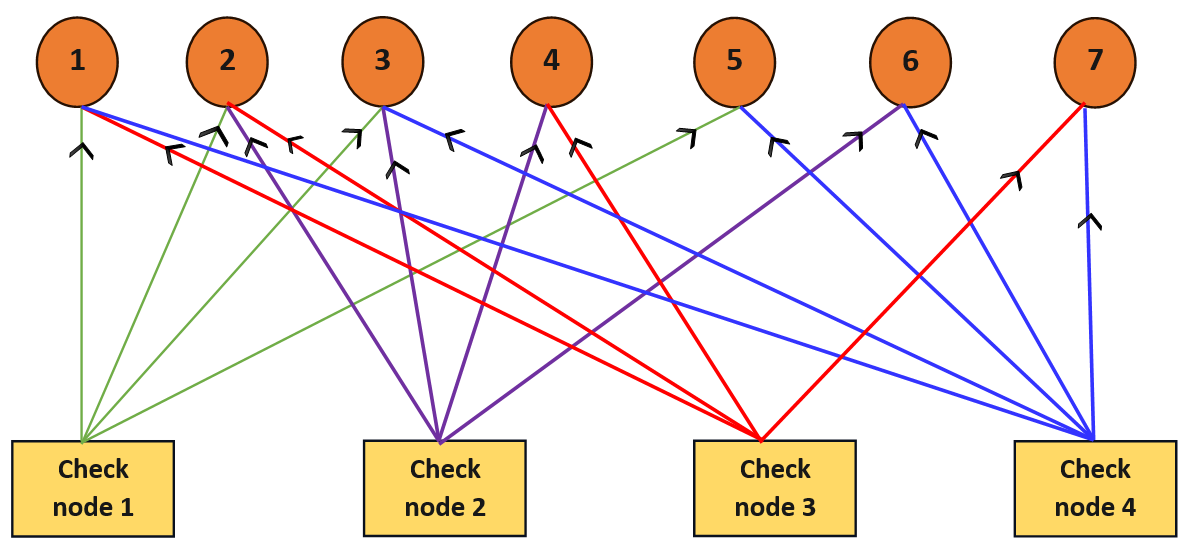
\includegraphics[width=0.55\textwidth]{48.png}
\end{figure*}

\textbf{4- Iteration:}\\ 
Steps 2 and 3 are repeated iteratively until convergence or for a fixed number of iterations. Convergence is typically determined by checking if there is no significant change in the messages between consecutive iterations.\\
Now we can say we know why it was called massage passing algorithm Because the messages (belief) are actually passed between Variable nodes and check nodes also we can call it belief propagation.\\
The steps required to implement MSA algorithm can be summarized in Figure~\ref{fig:MSA Algorithm}

\begin{figure}[ht]
    \centering
    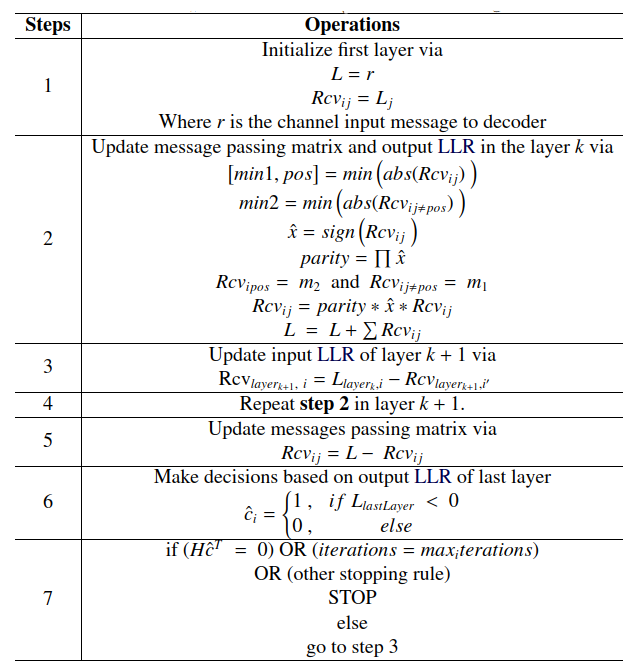
\includegraphics[width=0.85\textwidth]{image075.png}
    \caption{Steps for MSA Algorithm}
    \label{fig:MSA Algorithm}
\end{figure}

\subsubsection{Optimized Min-Sum Decoding Algorithm}
The outputs from variable nodes in MSA decoding are overestimated compared to SPA (sum of product algorithm) due to MSA uses  numerical approximation. There are several methods to optimize Min-Sum Algorithms (MSA) to make the approximation more accurate. The two most popular methods are Normalized Min-Sum Algorithm (NMSA) and Offset Min-Sum Algorithm (OMSA). The idea behind NMSA and OMSA is to reduce the magnitude of variable node.\\
Assume that the magnitudes of variable nodes output of MSA , NMSA and OMSA are $L^{MSA}$, $L^{NMSA}$, $L^{OMSA}$ \\
For Normalized Min-Sum Algorithm
\[ L^{NMSA}=\alpha L^{MSA} \]
Where $\alpha$ is called normalization factor and $0 < \alpha < 1$. \\
For Offset Min-Sum Algorithm,
\[ \ L^{OMSA}=\max\left(L^{MSA}-\beta,0\right) \]
Where $\beta$ is called offset factor and $\beta > 0$.

\subsubsection{Layered Message Passing Algorithm}
Suppose the parity check matrix H can be grouped into several subsets, and each subset follows the property that the column weight of each subset is at most 1 and one subset after another. In that case, layered decoding can be used. Layered message passing decoding can expedite convergence time. Because the check nodes operations can be processed when the variable nodes operations in one layer are done instead of waiting for all variable nodes operations in the whole parity-check matrix done.\\

The layered message passing can be illustrated using Figure 2.12. Each layer processes variable nodes operation and check nodes operation independently. The input LLR of the current layer is the output of previous LLR. Figure 3.12 shows layered message passing procedure of three layers. The initial LLR is assigned to Layer1. LLR1 is the output LLR of Layer1 and input LLR of Layer2. LLR2 is the output LLR of Layer2 and input LLR of Layer3. The output LLR of the last layer is the output LLR of the decoding algorithm and will be used to make the decision.
\begin{figure}[ht]
    \centering
    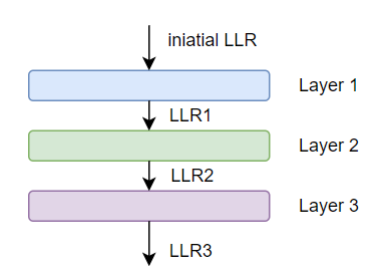
\includegraphics[width=0.5\textwidth]{image046.png}
    \caption{Layered message passing example}
    \label{fig:Layered message passing example }
\end{figure}
The variable nodes operation and check nodes operation in each layer are the same with  MSA. The difference is the updated LLR for each layer. The current layer input LLR can be updated.
\[ l_{layer_k+1,i}=L_{layer_k+1,i}-l_{layer_k+1,i^\prime} \]
Where $l_{layer_k+1,i}$ is the updated input LLR of layer $k+1$, $L_{layer_k+1,i}$ is the output LLR of previous layer , $l_{layer_k+1,i^\prime}$ is old input LLR of layer $k+1$.\\
\begin{GrayBox}
    \textbf{Note:} In order to apply the layered decoding algorithm, the parity check matrix must satisfy that in each layer the column weight is 1 and As we have seen in Figure~\ref{fig:H parity} this condition is met by 5G parity check matrix.
\end{GrayBox}
\textbf{Toy example for illustration:}\\
We will not use a 5G parity check matrix in our example because it is very large So here is the toy example we have split this parity check matrix into two layers, layer 1 and layer 2 and these are the two layers, okay we can see the first layer has just a single 1 in each column, (column weight is 1), similarly the second layer also has a column weight 1 these two together specify the overall parity check matrix.
\[ H=\left[\begin{matrix}1&1&1&0&1&0&0\\0&0&0&1&0&1&1\\\cdots&\cdots&\cdots&\cdots&\cdots&\cdots&\cdots\\1&1&0&1&0&0&1\\0&0&1&0&1&1&0\\\end{matrix}\right] \]
\textbf{1- Initialization Step}\\
We initialize only the first layer
\[  r=[\begin{matrix}0.2&-0.3&1.2&-0.5&0.8&0.6&-1.1\\\end{matrix}] \]
\[ L=\left[\begin{matrix}0.2&-0.3&1.2&0&0.8&0&0\\0&0&0&-0.5&0&0.6&-1.1\\\cdots&\cdots&\cdots&\cdots&\cdots&\cdots&\cdots\\\blacksquare&\blacksquare&0&\blacksquare&0&0&\blacksquare\\0&0&\blacksquare&0&\blacksquare&\blacksquare&0\\\end{matrix}\right] \]
\textbf{2- Row Operation on Layer 1}\\
Min-Sum on row $1,2$ (first layer)\\
Iteration 1 layer 1:\\
\[ L=\left[\begin{matrix}0.2&-0.3&1.2&0&0.8&0&0\\0&0&0&-0.5&0&0.6&-1.1\\\cdots&\cdots&\cdots&\cdots&\cdots&\cdots&\cdots\\\blacksquare&\blacksquare&0&\blacksquare&0&0&\blacksquare\\0&0&\blacksquare&0&\blacksquare&\blacksquare&0\\\end{matrix}\right] \]
Min-sum on first layer: Row $1, 2$\\
\[ r=[\begin{matrix}0.2&-0.3&1.2&-0.5&0.8&0.6&-1.1\\\end{matrix}] \]
\[ L=\left[\begin{matrix}-0.3&0.2&-0.2&0&-0.2&0&0\\0&0&0&-0.6&0&0.5&-0.5\\\cdots&\cdots&\cdots&\cdots&\cdots&\cdots&\cdots\\\blacksquare&\blacksquare&0&\blacksquare&0&0&\blacksquare\\0&0&\blacksquare&0&\blacksquare&\blacksquare&0\\\end{matrix}\right] \]
\textbf{3- Update The Messages (Column Operation)}\\
So first step was initialization, second step was this min sum which we did in layer 1 for iteration 1, and then we immediately update messages,
$\text{Sum} j = r j + \text{entry in Column}$
Here we update massages not after one iteration but after only one layer and this explains why layered MSA  converge faster than MSA
\[ \text{Sum} = [\begin{matrix}-0.1&-0.1&1&-0.1&0.6&1.1&-1.6\\\end{matrix}] \]
\textbf{4- Layer 2 Initialization}\\
Now that layer 1 is done and we will use the output beliefs (massages) from layer 1 as a input beliefs (massages) for  layer 2. And then we will do same.
Then we will apply the same operations that we did in the first layer to the second layer
\begin{enumerate}
    \item Initialization step.
    \item Row operation on layer 2 (Min Sum)
    \item Update the messages (column operation)
\end{enumerate}
Iteration 1, layer 2 initialization:
\[ \text{Sum} =  [\begin{matrix}-0.1&-0.1&1&-0.1&0.6&1.1&-1.6\\\end{matrix}] \]
\[ L=\left[\begin{matrix}-0.3&0.2&-0.2&0&-0.2&0&0\\0&0&0&-0.6&0&0.5&-0.5\\\cdots&\cdots&\cdots&\cdots&\cdots&\cdots&\cdots\\-0.1&-0.1&0&-0.1&0&0&-1.6\\0&0&0.6&0&0.6&1.1&0\\\end{matrix}\right] \]
Min sum on layer 2: Rows $3, 4$
\[ \text{Sum} =  [\begin{matrix}-0.1&-0.1&1&-1.1&0.6&1.1&-1.6\\\end{matrix}] \]
\[ L=\left[\begin{matrix}-0.3&0.2&-0.2&0&-0.2&0&0\\0&0&0&-0.6&0&0.5&-0.5\\\cdots&\cdots&\cdots&\cdots&\cdots&\cdots&\cdots\\-0.1&-0.1&0&-0.1&0&0&-0.1\\0&0&0.6&0&1&0.6&0\\\end{matrix}\right] \]
Then we will update our beliefs.
\[ \text{Sum} = [\begin{matrix}-0.2&-0.2&1.6&-1.2&1.6&1.7&-1.7\\\end{matrix}] \]
\textbf{5- Iteration 2}\\
We will do same operations that we did in iteration 1 but there will be one minor difference in the next iteration because already $L$ matrix have some values, okay so what do we do in this case? the first step is we will subtract,
incoming beliefs from previous round has to be subtracted out before we do fresh processing and this step is very important, if we do not do this correctly a lot of instability will happen in our decoder because the incoming belief actually had some input from layer 1 itself in the previous iteration there was some input from layer 1 which was used in updating incoming belief so, we have to subtract this influence to avoid resend or reuse information.\\
Iteration 2, layer 1,subtraction:
\[ \text{Sum} = [\begin{matrix}-0.2&-0.2&1.6&-1.2&1.6&1.7&-1.7\\\end{matrix}] \]
\[ L=\left[\begin{matrix}-0.3&0.2&-0.2&0&-0.2&0&0\\0&0&0&-0.6&0&0.5&-0.5\\\cdots&\cdots&\cdots&\cdots&\cdots&\cdots&\cdots\\-0.1&-0.1&0&-0.1&0&0&-0.1\\0&0&0.6&0&1&0.6&0\\\end{matrix}\right] \]
After subtraction (sum$-L$):
\[ \text{Sum} =  [\begin{matrix}0.1&-0.4&1.8&-0.6&1.8&1.2&-1.2\\\end{matrix}] \]
Then initialization for layer 1:
\[ L=\left[\begin{matrix}0.1&-0.4&1.8&0&1.8&0&0\\0&0&0&-0.6&0&1.2&-1.2\\\cdots&\cdots&\cdots&\cdots&\cdots&\cdots&\cdots\\-0.1&-0.1&0&-0.1&0&0&-0.1\\0&0&0.6&0&1&0.6&0\\\end{matrix}\right] \]
Then we will do same operations that we did in iteration 1.\\
Iteration 2, layer 1: Min-sum \\
After layer 1 row operation:
\[ L=\left[\begin{matrix}-0.4&0.1&-0.1&0&-0.1&0&0\\0&0&0&-1.2&0&0.6&-0.6\\\cdots&\cdots&\cdots&\cdots&\cdots&\cdots&\cdots\\-0.1&-0.1&0&-0.1&0&0&-0.1\\0&0&0.6&0&1&0.6&0\\\end{matrix}\right] \]
Then Update in Layer 1 : Rows $1,2$ $(Sum_{new} = sum_{old}+ entry in column)$
\[ \text{Sum} = [\begin{matrix}0.1&-0.4&1.8&-0.6&1.8&1.2&-1.2\\\end{matrix}] \]
\[ L=\left[\begin{matrix}-0.4&0.1&-0.1&0&-0.1&0&0\\0&0&0&-1.2&0&0.6&-0.6\\\cdots&\cdots&\cdots&\cdots&\cdots&\cdots&\cdots\\-0.1&-0.1&0&-0.1&0&0&-0.1\\0&0&0.6&0&1&0.6&0\\\end{matrix}\right] \]
\[ \text{Sum}_{new} =  [\begin{matrix}-0.3&-0.3&1.7&-1.8&1.7&1.8&-1.8\\\end{matrix}] \]
Like we did in the first layer, when we found that the L matrix already had values, we do subtraction operation it to avoid resend or reuse information we will do same operations that we did in layer 1.\\
Iteration 2, layer 2 : Subtraction
\[ \text{Sum} =  [\begin{matrix}-0.3&-0.3&1.7&-1.8&1.7&1.8&-1.8\\\end{matrix}] \]
\[ L=\left[\begin{matrix}-0.4&0.1&-0.1&0&-0.1&0&0\\0&0&0&-1.2&0&0.6&-0.6\\\cdots&\cdots&\cdots&\cdots&\cdots&\cdots&\cdots\\-0.1&-0.1&0&-0.1&0&0&-0.1\\0&0&0.6&0&1&0.6&0\\\end{matrix}\right] \]
Subtraction in Layer 2: Rows $3,4$
\[ \text{Sum} =  [\begin{matrix}-0.2&-0.2&1.1&-1.7&0.7&1.2&-1.7\\\end{matrix}] \]
\[ L=\left[\begin{matrix}-0.4&0.1&-0.1&0&-0.1&0&0\\0&0&0&-1.2&0&0.6&-0.6\\\cdots&\cdots&\cdots&\cdots&\cdots&\cdots&\cdots\\-0.2&-0.2&0&-1.7&0&0&-1.7\\0&0&1.1&0&0.7&1.2&0\\\end{matrix}\right] \]
Iteration 2, layer 2: Min-sum
\[ \text{Sum} = [\begin{matrix}-0.2&-0.2&1.1&-1.7&0.7&1.2&-1.7\\\end{matrix}] \]
\[ L=\left[\begin{matrix}-0.4&0.1&-0.1&0&-0.1&0&0\\0&0&0&-1.2&0&0.6&-0.6\\\cdots&\cdots&\cdots&\cdots&\cdots&\cdots&\cdots\\-0.2&-0.2&0&-1.7&0&0&-1.7\\0&0&1.1&0&0.7&1.2&0\\\end{matrix}\right] \]
Min-sum in layer 2 :Rows $3,4$
\[ L=\left[\begin{matrix}-0.4&0.1&-0.1&0&-0.1&0&0\\0&0&0&-1.2&0&0.6&-0.6\\\cdots&\cdots&\cdots&\cdots&\cdots&\cdots&\cdots\\-0.2&-0.2&0&-0.2&0&0&-0.2\\0&0&0.7&0&1.1&0.7&0\\\end{matrix}\right] \]
Iteration 2, layer 2 : Update
\[ \text{Sum} = [\begin{matrix}-0.2&-0.2&1.1&-1.7&0.7&1.2&-1.7\\\end{matrix}] \]
Update in Layer 2 : Rows $3,4$
\[ L=\left[\begin{matrix}-0.4&0.1&-0.1&0&-0.1&0&0\\0&0&0&-1.2&0&0.6&-0.6\\\cdots&\cdots&\cdots&\cdots&\cdots&\cdots&\cdots\\-0.2&-0.2&0&-0.2&0&0&-0.2\\0&0&0.7&0&1.1&0.7&0\\\end{matrix}\right] \]
\[ \text{Sum} = [\begin{matrix}-0.4&-0.4&1.8&-1.9&1.8&1.9&-1.9\\\end{matrix}] \]
Now time for hard decision:
\begin{equation*}
    \text{BPSK}
    \begin{cases}
        1, & c=0 \\
        -1, & c=1
    \end{cases}
\end{equation*}
If Sum$ > 0$, Decision on Bit $j = 0$, If Sum$ < 0$, Decision on Bit $j = 1$.
\[ \text{Sum} = [\begin{matrix}-0.4&-0.4&1.8&-1.9&1.8&1.9&-1.9\\\end{matrix}] \]
\[ \begin{matrix}\text{DEC}=[1&1&0&1&0&0&1\\\end{matrix}] \]
\begin{GrayBox}
    \textbf{The operations that we do in LMSA can be summarized as:}\\
    Subtraction $\rightarrow$ Min-Sum $\rightarrow$ Update
\end{GrayBox}
In our project, we have implemented LOMSA to avoid over estimation of MSA we implement  offset min sum algorithm to reduce the magnitude of variable node and layered MSA to expedite convergence time. \\
The steps required to implement Layered Normalized Min-Sum Algorithm and Layered Offset Min-Sum Algorithm can be summarized in Figure~\ref{fig:LOMSA Algorithm}
\begin{figure}[ht]
    \centering
    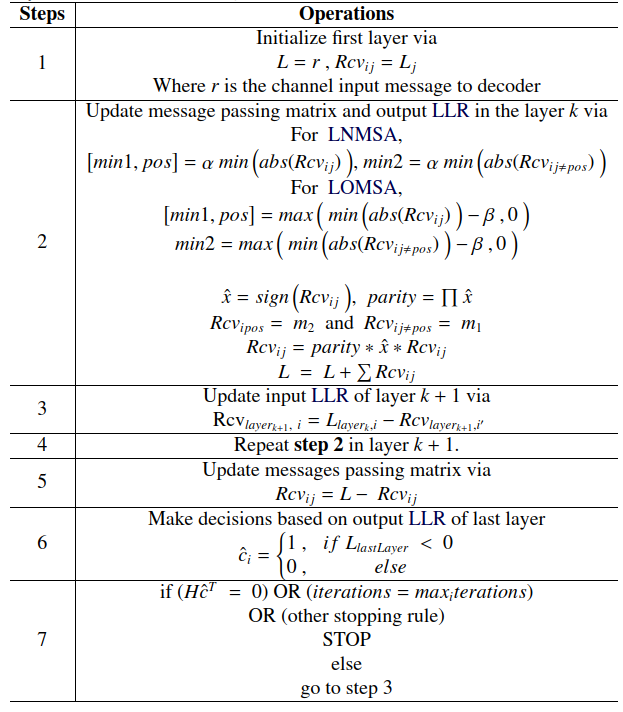
\includegraphics[width=0.85\textwidth]{image077.png}
    \caption{Implementation steps of LNMSA and LOMSA}
    \label{fig:LOMSA Algorithm}
\end{figure}
